\documentclass[12pt,letterpaper]{article}

% Packages
\usepackage[utf8]{inputenc}
\usepackage[T1]{fontenc}
\usepackage{amsmath, amssymb, amsfonts}
\usepackage{graphicx}
\usepackage{float}
\usepackage{placeins}
\usepackage{setspace}
\usepackage{enumitem}
\usepackage{authblk}
\usepackage{parskip}
\usepackage{xcolor}
\usepackage{textcomp}
\usepackage{siunitx}
\usepackage{hyperref}
\usepackage{geometry}
\usepackage{natbib}
\usepackage{booktabs}
\usepackage{caption}
\usepackage{subcaption}
\geometry{margin=1in}

% Custom colors and hyperlinks
\definecolor{linkcolor}{RGB}{0, 90, 160}
\hypersetup{
    colorlinks=true,
    linkcolor=linkcolor,
    urlcolor=linkcolor,
    citecolor=linkcolor
}

% Custom commands
\newcommand{\E}{\mathbb{E}}
\renewcommand{\P}{\mathbb{P}}
\newcommand{\V}{\text{Var}}

\title{A Run Expectancy Approach to Lead Distance Optimization in Major League Baseball}

\author[1]{Jack Whitney-Epstein}
\author[2]{Zach Sissman}
\author[3]{Lila Dodson}

% Affiliations
\affil[1]{\small The Brunswick School, Greenwich, CT}
\affil[2]{\small Community School of Naples, Naples, FL}
\affil[3]{\small San Francisco University High School, San Francisco, CA}

\date{\today}

\begin{document}

\maketitle

\begin{abstract}
A runner's primary lead off first base creates a trade-off: a larger lead improves the runner's chance of stealing second but also increases exposure to pickoff attempts. Using 2024 MLB pitch-level data and Baseball Savant tracking measures, we model this trade-off as a sequential process with four stages: pickoff attempt, pickoff success conditional on an attempt, steal attempt conditional on no pickoff, and steal success conditional on an attempt. Each stage is estimated with logistic or mixed-effects logistic regression using lead distance, pitcher hold quality, runner sprint speed, catcher pop time, disengagement state, and outs, with runner and catcher random effects where appropriate. We then map the fitted stage probabilities to outs-specific RE24 run values and choose the lead distance that maximizes expected runs for each pitcher--catcher--runner context. Observed leads are slightly larger than the model-implied optimum on average: +0.13 ft across all runner-on-first pitches and +0.10 ft on steal attempts. The framework converts the steal--pickoff trade-off into a common run-expectancy scale and provides context-specific lead recommendations.
\end{abstract}

\section{Introduction}

\subsection{History of Base Stealing}

In baseball, scouts traditionally evaluate five tools: hitting for average, hitting for power, fielding, throwing, and speed. Among these, speed is often undervalued, despite playing a central role in a player's effectiveness on the basepaths. Stolen bases are the most visible expression of that impact.

Historically, steals have waxed and waned with MLB's run-scoring environment. During the Deadball era (c. 1900--1920), home run rates were low and teams relied more on advancing runners through stolen bases. Many seasons saw clubs exceed 100 steals and leagues tally well over 1,000 steals combined \citep{McMurray2015Deadball}. As home runs rose from the 1930s through the 1950s, average team steals fell to roughly 39 per season \citep{BaseballReference1950}. From the 1960s to the 1980s, players such as Lou Brock and Rickey Henderson brought base-stealing back into prominence. Maury Wills's 1962 season, which included 104 stolen bases, was a turning point in baserunning and influenced how opponents pitched and held runners on \citep{Vazzana2016MauryWills}.

\subsection{Sabermetrics and Expected Runs}

By the 1990s and 2000s, sabermetrics reframed the value of the steal. Bill James argued that a steal must succeed about two-thirds of the time to break even, a rule of thumb that recognizes outs as scarce resources and emphasizes efficiency over raw totals \citep{James2023Baserunning}. Building on this logic, linear weights assign average run values to outcomes independent of specific context. On Baseball Savant, a successful steal is valued at +0.20 expected runs, while being caught stealing or picked off is valued at -0.45 expected runs \citep{BaseballSavantRunValueND}. These values provide a useful baseline for evaluation.

However, context still matters when deciding whether to steal. The run value of a steal depends on the base-out state, defined by which bases are occupied and the number of outs. There are $2^3 \times 3 = 24$ possible base-out states. Sabermetrics defines the value of a play as the change in run expectancy between states, and run expectancy tables such as Table~\ref{tab:re24} are commonly used to estimate this value. According to Table~\ref{tab:re24}, stealing second base with 0 outs and no other runners on base is worth $1.068 - 0.831 = 0.237$ runs, while being caught stealing in the same situation is worth $0.243 - 0.831 = -0.588$ runs \citep{FanGraphsRE24ND}.

\begin{table}[htbp]
\centering
\caption{Example run expectancy table}
\label{tab:re24}
\begin{tabular}{l S S S}
\toprule
\textbf{Runners} & {\textbf{0 Outs}} & {\textbf{1 Out}} & {\textbf{2 Outs}}\\
\midrule
Empty   & 0.461 & 0.243 & 0.095 \\
$1\ \_\,\_$ & 0.831 & 0.489 & 0.214 \\
$\_\,2\ \_$ & 1.068 & 0.644 & 0.305 \\
$1\ 2\ \_$  & 1.373 & 0.908 & 0.343 \\
$\_\,\_\,3$ & 1.426 & 0.865 & 0.413 \\
$1\ \_\,3$  & 1.798 & 1.140 & 0.471 \\
$\_\,2\ 3$  & 1.920 & 1.352 & 0.570 \\
$1\ 2\ 3$   & 2.282 & 1.520 & 0.736 \\
\bottomrule
\end{tabular}

\vspace{0.25em}
\footnotesize Example run expectancy table \citep{FanGraphsRE24ND}.
\end{table}

\subsection{The Lead's Impact on Base Stealing}

While speed is a key ingredient in stealing bases, the lead a runner takes off first base also shapes both steal success and pickoff risk. A larger lead shortens the distance to second if the runner goes, but it also increases exposure to pickoff attempts at first.

This strategic dimension of stealing has been studied in game-theoretic terms. \citet{Turocy2014Theft} models the steal decision as a two-player inspection game between the runner and the defense, where the runner chooses whether to go and the defense allocates attention between the runner and the batter. The mixed-strategy equilibrium implies a near-linear relationship between attempt frequency and success rate, with validation over MLB play-by-play data from 1974--2011. However, the framework does not prescribe an optimal primary lead or incorporate pitcher- and catcher-specific skills at the pitch level.

A complementary physics approach examines the kinematics of a steal attempt. Using position--time and velocity--time profiles for a case study, \citet{Kagan2013StolenBasePhysics} parametrizes acceleration from first, slide deceleration, top speed, speed upon arrival, and the runner's lead distance. He finds that sprint speed and initial acceleration most strongly affect success, with comparatively modest effects attributed to the primary lead. This analysis is mechanically useful, but it only implicitly considers pickoff risk and is limited in scope.

Data-driven work using tracking-era measurements shows how player behavior and pitcher tendencies shape leads. \citet{Lindbergh2015Statcast} uses MLB data on primary and secondary leads and sprint speed, highlighting outliers such as Jon Lester's reluctance to throw over and Ichiro Suzuki's larger-than-expected leads relative to speed. That study also notes a positive association between sprint speed and lead size. It does not, however, jointly model runner, pitcher, and catcher characteristics, nor does it connect the full decision sequence from pickoff attempt to steal outcome to expected runs.

This study extends the existing literature in four ways. First, we model the baserunning sequence with a nested set of logistic regressions. Second, we incorporate runner sprint speed, pitcher hold ability (\emph{Threat}), catcher pop time, disengagement state, and outs in the relevant stages. Third, we use random effects to account for unobserved runner and catcher heterogeneity. Fourth, we optimize primary lead distance to maximize expected runs for the base state with a runner on first and second and third base empty. In doing so, we quantify the reward of a larger lead and the cost of greater pickoff risk on a common run-expectancy scale.

\section{Methodology}

\subsection{Data Overview}

Our primary dataset, provided by MLB, consists of 2024 pitch-level observations. It includes all pickoff attempts, a random sample of called pitches, and every stolen-base attempt on takes, defined as pitches where the batter did not swing. The unit of observation is a single pitch. Each observation includes pitch context (inning, date, home/away, count, and outs), participant IDs (runner, pitcher, and catcher), and the runner's primary and secondary lead distances in feet. We denote the primary lead by $L_i$. To avoid base-state confounding, we restrict the analysis to the state with a runner on first and second and third base empty. Under this restriction, the only base-out component that varies in the run-expectancy calculation is the number of outs.

We merge the pitch-level data with the following covariates from Baseball Savant:
\begin{itemize}
    \item Runner sprint speed, $v_i$ (feet per second).
    \item Catcher pop time, $p_i$ (seconds), defined as the average time it takes a catcher to throw the ball to second base after receiving a pitch.
    \item Pitcher \emph{Threat}, $\theta_i$ (per 100 IP): Baseball Savant's Net Bases Prevented \citep{BaseballSavantRunValueND} scaled to 100 innings pitched, $\theta_i = 100\,\mathrm{NBP}/\mathrm{IP}$. Higher values indicate stronger control of the running game.
    \item Disengagement state, $r_i \in \{0,1,2\}$, an indicator capturing the 2023 MLB rule limiting pickoff attempts. Under this rule, a pitcher is allowed two pickoffs or step-offs per plate appearance; a third disengagement results in a balk unless the runner is successfully picked off. Since we do not observe step-offs, we construct this variable using only observed pickoff attempts: $r_i=0$ indicates no prior pickoffs, $r_i=1$ indicates one prior pickoff, and $r_i=2$ indicates two or more prior pickoff attempts.
    \item Outs, $o_i \in \{0,1,2\}$.
\end{itemize}

All continuous predictors (lead distance, pitcher Threat, catcher pop time, and runner sprint speed) are standardized by subtracting their sample mean and dividing by their sample standard deviation. This places predictors on comparable scales. In the logistic models below, each continuous coefficient represents the change in log-odds associated with a one-standard-deviation increase in the predictor.

To evaluate the expected value of base-stealing outcomes, we use situational weights derived from the RE24 run expectancy table (Table~\ref{tab:re24}):
\begin{equation}
    \mathrm{xRuns}_i = w_{\mathrm{SB}}(o_i) \cdot \mathbf{1}\{\mathrm{SB}_i\}
    + w_{\mathrm{CS}}(o_i) \cdot \mathbf{1}\{\mathrm{CS}_i\}
    + w_{\mathrm{PK}}(o_i) \cdot \mathbf{1}\{\mathrm{PK}_i\}. \label{eq:xRuns}
\end{equation}
Here $w_{\mathrm{SB}}(o_i)$, $w_{\mathrm{CS}}(o_i)$, and $w_{\mathrm{PK}}(o_i)$ are the changes in run expectancy associated with a stolen base, caught stealing, and pickoff, respectively, given the current number of outs. Because the analysis is restricted to runner on first with second and third empty, these weights vary only by outs.

\subsection{Modeling Framework}

We represent the runner-on-first sequence as a set of conditional events. First, the pitcher may attempt a pickoff. Conditional on a pickoff attempt, the runner may be picked off. If no pickoff is attempted, the runner may attempt to steal. Conditional on a steal attempt, the steal may succeed. Pitches on which none of these events occur are classified as no-event pitches and receive zero incremental run value in Equation~\ref{eq:xRuns}.

We model the pickoff-attempt stage with a fixed-effects logistic regression and the pickoff-success, steal-attempt, and steal-success stages with mixed-effects logistic regressions. Random intercepts are included for runners in the pickoff-success stage and for both runners and catchers in the steal-attempt and steal-success stages. Outs enters the pickoff-attempt, steal-attempt, and steal-success stages directly as a predictor; it also enters the expected-runs objective through the outs-specific RE24 weights. Formally,
\begin{align}
    \P(\mathrm{PO}_i \mid L_i, \theta_i, r_i, o_i)
    &= \mathrm{logit}^{-1}(\alpha_0 + \alpha_1 L_i + \alpha_2 \theta_i + \alpha_3 r_i + \alpha_4 o_i), \label{eq:node-1} \\
    \P(\mathrm{PK}_i \mid \mathrm{PO}_i, L_i, \theta_i, r_i)
    &= \mathrm{logit}^{-1}(\beta_0 + \beta_1 L_i + \beta_2 \theta_i + \beta_3 r_i + u_{i,\mathrm{PK}}), \label{eq:node-2} \\
    \P(\mathrm{ATT}_i \mid \neg\mathrm{PO}_i, \theta_i, p_i, v_i, r_i, o_i)
    &= \mathrm{logit}^{-1}(\gamma_0 + \gamma_1 \theta_i + \gamma_2 p_i + \gamma_3 v_i + \gamma_4 r_i + \gamma_5 o_i 
    + u_{i,\mathrm{ATT}} + z_{i,\mathrm{ATT}}), \label{eq:node-3} \\
    \P(\mathrm{SB}_i \mid \mathrm{ATT}_i, L_i, \theta_i, p_i, v_i, r_i, o_i)
    &= \mathrm{logit}^{-1}(\delta_0 + \delta_1 L_i + \delta_2 \theta_i + \delta_3 p_i + \delta_4 v_i 
    + \delta_5 r_i + \delta_6 o_i + u_{i,\mathrm{SB}} + z_{i,\mathrm{SB}}). \label{eq:node-4}
\end{align}
Here $u_{i,\cdot}$ and $z_{i,\cdot}$ denote runner- and catcher-specific random intercept terms for the corresponding stages. The notation $r_i$ and $o_i$ in Equations~\ref{eq:node-1}--\ref{eq:node-4} is shorthand for categorical fixed effects, with 0 prior disengagements and 0 outs used as the reference levels.

We exclude outs from the pickoff-success-given-attempt stage. Once a throw-over occurs, pickoff success is more directly tied to lead distance, pitcher move quality, runner traits, and disengagement context than to the base-out valuation. This restriction also keeps the pickoff-success stage parsimonious, since successful pickoffs are relatively rare.

We also exclude primary lead distance from the steal-attempt model. This treats the attempt model as capturing the runner's baseline green-light tendency after conditioning on pitcher, catcher, runner, disengagement state, and outs. Including lead distance in this stage would risk using the runner's realized pre-pitch positioning as a proxy for unobserved steal intent, which would partially absorb the effect of lead distance that the optimization is designed to study.

Let $X_i=(\theta_i,p_i,v_i,r_i,o_i)$ represent the observed player characteristics and game context for pitch $i$. The unconditional stage probabilities are then
\begin{align*}
    \P(\mathrm{PK}_i \mid L_i, X_i)
    &= \P(\mathrm{PK}_i \mid \mathrm{PO}_i, L_i, \theta_i, r_i)\cdot
       \P(\mathrm{PO}_i \mid L_i, \theta_i, r_i, o_i), \\
    \P(\mathrm{ATT}_i \mid L_i, X_i)
    &= \P(\mathrm{ATT}_i \mid \neg\mathrm{PO}_i, \theta_i, p_i, v_i, r_i, o_i)\cdot
       \bigl(1-\P(\mathrm{PO}_i \mid L_i, \theta_i, r_i, o_i)\bigr), \\
    \P(\mathrm{SB}_i \mid L_i, X_i)
    &= \P(\mathrm{SB}_i \mid \mathrm{ATT}_i, L_i, X_i)\cdot
       \P(\mathrm{ATT}_i \mid L_i, X_i), \\
    \P(\mathrm{CS}_i \mid L_i, X_i)
    &= \bigl(1-\P(\mathrm{SB}_i \mid \mathrm{ATT}_i, L_i, X_i)\bigr)\cdot
       \P(\mathrm{ATT}_i \mid L_i, X_i).
\end{align*}

Taking conditional expectations of Equation~\ref{eq:xRuns} gives
\begin{align}
    \E[\mathrm{xRuns}_i \mid L_i, X_i]
    &= w_{\mathrm{SB}}(o_i) \cdot \P(\mathrm{SB}_i \mid L_i, X_i)
    + w_{\mathrm{CS}}(o_i) \cdot \P(\mathrm{CS}_i \mid L_i, X_i) \nonumber \\
    &\quad + w_{\mathrm{PK}}(o_i) \cdot \P(\mathrm{PK}_i \mid L_i, X_i). \label{eq:xRuns-estimable}
\end{align}
Thus, the expected run value of a candidate lead is estimable from the four fitted stage models and the outs-specific RE24 weights.

\subsection{Objective and Optimization}

For each fixed context $X_i=(\theta_i,p_i,v_i,r_i,o_i)$, we evaluate the expected run value of candidate primary leads using Equation~\ref{eq:xRuns-estimable}. The model-implied optimal lead is
\begin{equation}
    L_i^* = \underset{L\in\mathcal{L}}{\arg\max}\ \mathrm{xRuns}(L\mid X_i), \label{eq:optimization}
\end{equation}
where $\mathcal{L}$ denotes the candidate lead range. In implementation, $\mathcal{L}=[0,90]$ is used as a broad numerical bound for optimization, not as a physically meaningful range of feasible primary leads. Substantive interpretations are restricted to optima that fall within the empirically relevant range of observed primary leads.

We solve Equation~\ref{eq:optimization} using R's \texttt{optimize()} function, which implements Brent's method \citep{Brent1973}. Because any optimum selected near the boundary of the candidate range would depend heavily on extrapolation, such cases should be treated as diagnostic rather than as actionable recommendations. We compare observed leads to $L_i^*$ to summarize how far runners are from the model-implied optimum.

\section{Results}

\subsection{Model Estimates} \label{sec:model-estimates}

We report coefficient estimates for the logistic and mixed-effects logistic regressions in Tables~\ref{tab:po}--\ref{tab:sb_att}. All interpretations below are associative rather than causal, conditional on the included covariates and model specification. The fitted models recover the expected qualitative trade-off: larger leads are associated with both more pickoff attempts and substantially higher pickoff success conditional on an attempt, while also being associated with higher steal success conditional on a steal attempt.

In the pickoff-attempt model (Table~\ref{tab:po}), a one-standard-deviation increase in lead distance is associated with roughly 36\% higher odds of a throw-over ($\exp(0.309)\approx1.36$), while a one-standard-deviation increase in pitcher \emph{Threat} is associated with roughly 5\% lower odds of a pickoff attempt ($\exp(-0.052)\approx0.95$). After one prior pickoff attempt, the odds of attempting another pickoff increase by about 75\% ($\exp(0.561)\approx1.75$). After two prior pickoff attempts, the odds increase by about 65\% ($\exp(0.502)\approx1.65$). Relative to 0 outs, 1 out is associated with higher pickoff-attempt odds ($\exp(0.092)\approx1.10$), while the 2-outs contrast is not statistically distinguishable from zero.

In the pickoff-success-given-attempt model (Table~\ref{tab:pk_po}), a one-standard-deviation increase in lead distance is associated with roughly 186\% higher odds of pickoff success ($\exp(1.050)\approx2.86$), while a one-standard-deviation increase in pitcher \emph{Threat} is associated with roughly 121\% higher odds ($\exp(0.791)\approx2.21$). After one prior pickoff attempt, the odds of a successful pickoff increase by about 68\% ($\exp(0.518)\approx1.68$). After two prior pickoff attempts, the effect is not statistically significant ($p=0.112$). The runner-specific random effect shows substantial individual variation (variance = 0.444, SD = 0.666), suggesting that some runners are more vulnerable to being picked off after conditioning on the observed covariates.

In the steal-attempt-given-no-pickoff model (Table~\ref{tab:att_no_po}), a one-standard-deviation increase in \emph{Threat} is associated with roughly 38\% lower odds of a steal attempt ($\exp(-0.471)\approx0.62$). Attempt odds are higher with slower catchers (about 6\% per standard deviation; $\exp(0.060)\approx1.06$) and faster runners (about 145\% per standard deviation; $\exp(0.896)\approx2.45$). After one prior pickoff attempt, steal-attempt odds increase by about 145\% ($\exp(0.898)\approx2.46$). After two prior pickoff attempts, attempt odds increase by about 290\% ($\exp(1.360)\approx3.90$). Outs is also a strong predictor in this stage: relative to 0 outs, attempt odds are about 37\% higher at 1 out ($\exp(0.317)\approx1.37$) and about 94\% higher at 2 outs ($\exp(0.664)\approx1.94$). Random effects show substantial runner heterogeneity (variance = 0.523, SD = 0.723) and smaller but nonzero catcher heterogeneity (variance = 0.014, SD = 0.117).

In the steal-success-given-attempt model (Table~\ref{tab:sb_att}), a one-standard-deviation increase in lead distance is associated with roughly 16\% higher odds of success ($\exp(0.148)\approx1.16$), while a one-standard-deviation increase in pitcher \emph{Threat} is associated with roughly 25\% lower odds ($\exp(-0.286)\approx0.75$). Success odds are also higher with slower catcher pop times (about 33\% per standard deviation; $\exp(0.286)\approx1.33$). Sprint speed shows a marginal positive association ($p=0.071$), disengagement-stage effects are not statistically significant, and the outs terms are not statistically significant in this stage. Random effects remain modest (runner variance = 0.127, catcher variance = 0.011), suggesting that much of the observed variation in steal success is captured by the included situational variables.

Overall, these associations align with baseball intuition and indicate that the model stack captures the intended trade-off between lead size, pickoff risk, and steal success. The probability estimates should be interpreted as model-implied quantities for the analyzed pitch sample rather than as definitive causal effects.

\begin{table}[htbp]
\centering
\caption{Logistic regression for pickoff attempts (PO)}
\label{tab:po}
\begin{tabular}{lrrrr}
\toprule
\multicolumn{5}{c}{\textbf{Fixed Effects}} \\
\midrule
Term & Estimate & Std. Error & z value & Pr($>|z|$) \\
\midrule
(Intercept)      & -2.3242 & 0.0244 & -95.142 & $< 2\times10^{-16}$ \\
lead\_scaled     &  0.3089 & 0.0121 &  25.477 & $< 2\times10^{-16}$ \\
threat\_scaled   & -0.0521 & 0.0118 &  -4.411 & $1.03\times10^{-5}$ \\
dis\_state1      &  0.5614 & 0.0343 &  16.366 & $< 2\times10^{-16}$ \\
dis\_state2      &  0.5017 & 0.0730 &   6.872 & $6.33\times10^{-12}$ \\
outs\_f1         &  0.0920 & 0.0311 &   2.963 & $3.05\times10^{-3}$ \\
outs\_f2         & -0.0192 & 0.0316 &  -0.606 & $5.44\times10^{-1}$ \\
\midrule
\multicolumn{5}{c}{\textbf{Random Effects}} \\
\midrule
\multicolumn{5}{l}{No random effects (fixed-effects GLM)} \\
\multicolumn{5}{l}{Number of obs: 72,645} \\
\bottomrule
\end{tabular}
\end{table}

\begin{table}[htbp]
\centering
\caption{Mixed-effects logistic regression for pickoff success given attempt (PK $\mid$ PO)}
\label{tab:pk_po}
\begin{tabular}{lrrrr}
\toprule
\multicolumn{5}{c}{\textbf{Fixed Effects}} \\
\midrule
Term & Estimate & Std. Error & z value & Pr($>|z|$) \\
\midrule
(Intercept)      & -5.2758 & 0.2266 & -23.278 & $< 2\times10^{-16}$ \\
lead\_scaled     &  1.0495 & 0.1125 &   9.327 & $< 2\times10^{-16}$ \\
threat\_scaled   &  0.7911 & 0.1198 &   6.602 & $4.07\times10^{-11}$ \\
dis\_state1      &  0.5181 & 0.2230 &   2.324 & $2.01\times10^{-2}$ \\
dis\_state2      &  0.6644 & 0.4176 &   1.591 & $1.12\times10^{-1}$ \\
\midrule
\multicolumn{5}{c}{\textbf{Random Effects}} \\
\midrule
\multicolumn{5}{l}{Runner1B\_ID (Intercept): Variance = 0.4440, SD = 0.6663} \\
\multicolumn{5}{l}{Number of obs: 7,439; groups (Runner1B\_ID): 530} \\
\bottomrule
\end{tabular}
\end{table}

\begin{table}[htbp]
\centering
\caption{Mixed-effects logistic regression for steal attempt given no pickoff (ATT $\mid \neg$PO)}
\label{tab:att_no_po}
\begin{tabular}{lrrrr}
\toprule
\multicolumn{5}{c}{\textbf{Fixed Effects}} \\
\midrule
Term & Estimate & Std. Error & z value & Pr($>|z|$) \\
\midrule
(Intercept)        & -4.4160 & 0.0667 & -66.223 & $< 2\times10^{-16}$ \\
threat\_scaled     & -0.4712 & 0.0173 & -27.323 & $< 2\times10^{-16}$ \\
poptime\_scaled    &  0.0600 & 0.0274 &   2.192 & $2.84\times10^{-2}$ \\
sprint\_scaled     &  0.8957 & 0.0486 &  18.424 & $< 2\times10^{-16}$ \\
dis\_state1        &  0.8983 & 0.0558 &  16.096 & $< 2\times10^{-16}$ \\
dis\_state2        &  1.3603 & 0.0984 &  13.822 & $< 2\times10^{-16}$ \\
outs\_f1           &  0.3169 & 0.0613 &   5.170 & $2.34\times10^{-7}$ \\
outs\_f2           &  0.6642 & 0.0592 &  11.221 & $< 2\times10^{-16}$ \\
\midrule
\multicolumn{5}{c}{\textbf{Random Effects}} \\
\midrule
\multicolumn{5}{l}{Runner1B\_ID (Intercept): Variance = 0.5233, SD = 0.7234} \\
\multicolumn{5}{l}{CatcherID (Intercept): Variance = 0.0136, SD = 0.1165} \\
\multicolumn{5}{l}{Number of obs: 65,206; groups (Runner1B\_ID): 602; CatcherID: 83} \\
\bottomrule
\end{tabular}
\end{table}

\begin{table}[htbp]
\centering
\caption{Mixed-effects logistic regression for steal success given attempt (SB $\mid$ ATT)}
\label{tab:sb_att}
\begin{tabular}{lrrrr}
\toprule
\multicolumn{5}{c}{\textbf{Fixed Effects}} \\
\midrule
Term & Estimate & Std. Error & z value & Pr($>|z|$) \\
\midrule
(Intercept)        &  0.8672 & 0.1320 &   6.572 & $4.96\times10^{-11}$ \\
lead\_scaled       &  0.1480 & 0.0652 &   2.268 & $2.33\times10^{-2}$ \\
threat\_scaled     & -0.2861 & 0.0493 &  -5.808 & $6.34\times10^{-9}$ \\
poptime\_scaled    &  0.2856 & 0.0545 &   5.242 & $1.59\times10^{-7}$ \\
sprint\_scaled     &  0.1175 & 0.0651 &   1.805 & $7.11\times10^{-2}$ \\
dis\_state1        & -0.1404 & 0.1209 &  -1.161 & $2.46\times10^{-1}$ \\
dis\_state2        & -0.1608 & 0.2026 &  -0.794 & $4.27\times10^{-1}$ \\
outs\_f1           &  0.0261 & 0.1359 &   0.192 & $8.48\times10^{-1}$ \\
outs\_f2           &  0.1899 & 0.1323 &   1.435 & $1.51\times10^{-1}$ \\
\midrule
\multicolumn{5}{c}{\textbf{Random Effects}} \\
\midrule
\multicolumn{5}{l}{Runner1B\_ID (Intercept): Variance = 0.1272, SD = 0.3567} \\
\multicolumn{5}{l}{CatcherID (Intercept): Variance = 0.0108, SD = 0.1039} \\
\multicolumn{5}{l}{Number of obs: 2,434; groups (Runner1B\_ID): 417; CatcherID: 83} \\
\bottomrule
\end{tabular}
\end{table}

\FloatBarrier

\subsection{Expected Runs and Lead Deviation}

For each pitcher--catcher--runner context $X_i=(\theta_i,p_i,v_i,r_i,o_i)$ and each candidate lead distance $L\in\mathcal{L}$, we compute $\mathrm{xRuns}(L\mid X_i)$ using Equation~\ref{eq:xRuns-estimable}. We then report the model-implied optimal lead as in Equation~\ref{eq:optimization}:
\[
    L_i^* = \underset{L\in\mathcal{L}}{\arg\max}\ \mathrm{xRuns}(L\mid X_i).
\]
We define lead deviation as
\begin{equation}
    d_i \equiv L_i^{\mathrm{obs}} - L_i^*. \label{eq:deviation}
\end{equation}
Positive values indicate observed leads that are larger than the model-implied optimum, while negative values indicate observed leads that are smaller. Across all runner-on-first observations, deviations are centered slightly above zero, with a mean of +0.13 ft (Figure~\ref{fig:deviation_all}). On steal attempts, the mean deviation remains positive but is smaller, +0.10 ft (Figure~\ref{fig:deviation_sba}). Thus, runners in this sample tend to take slightly more aggressive leads than the model recommends, though the average difference is small relative to typical primary lead distances.

Additional visualizations of lead deviation are included in Appendix~\ref{app:a}.

\begin{figure}[!htbp]
    \centering
    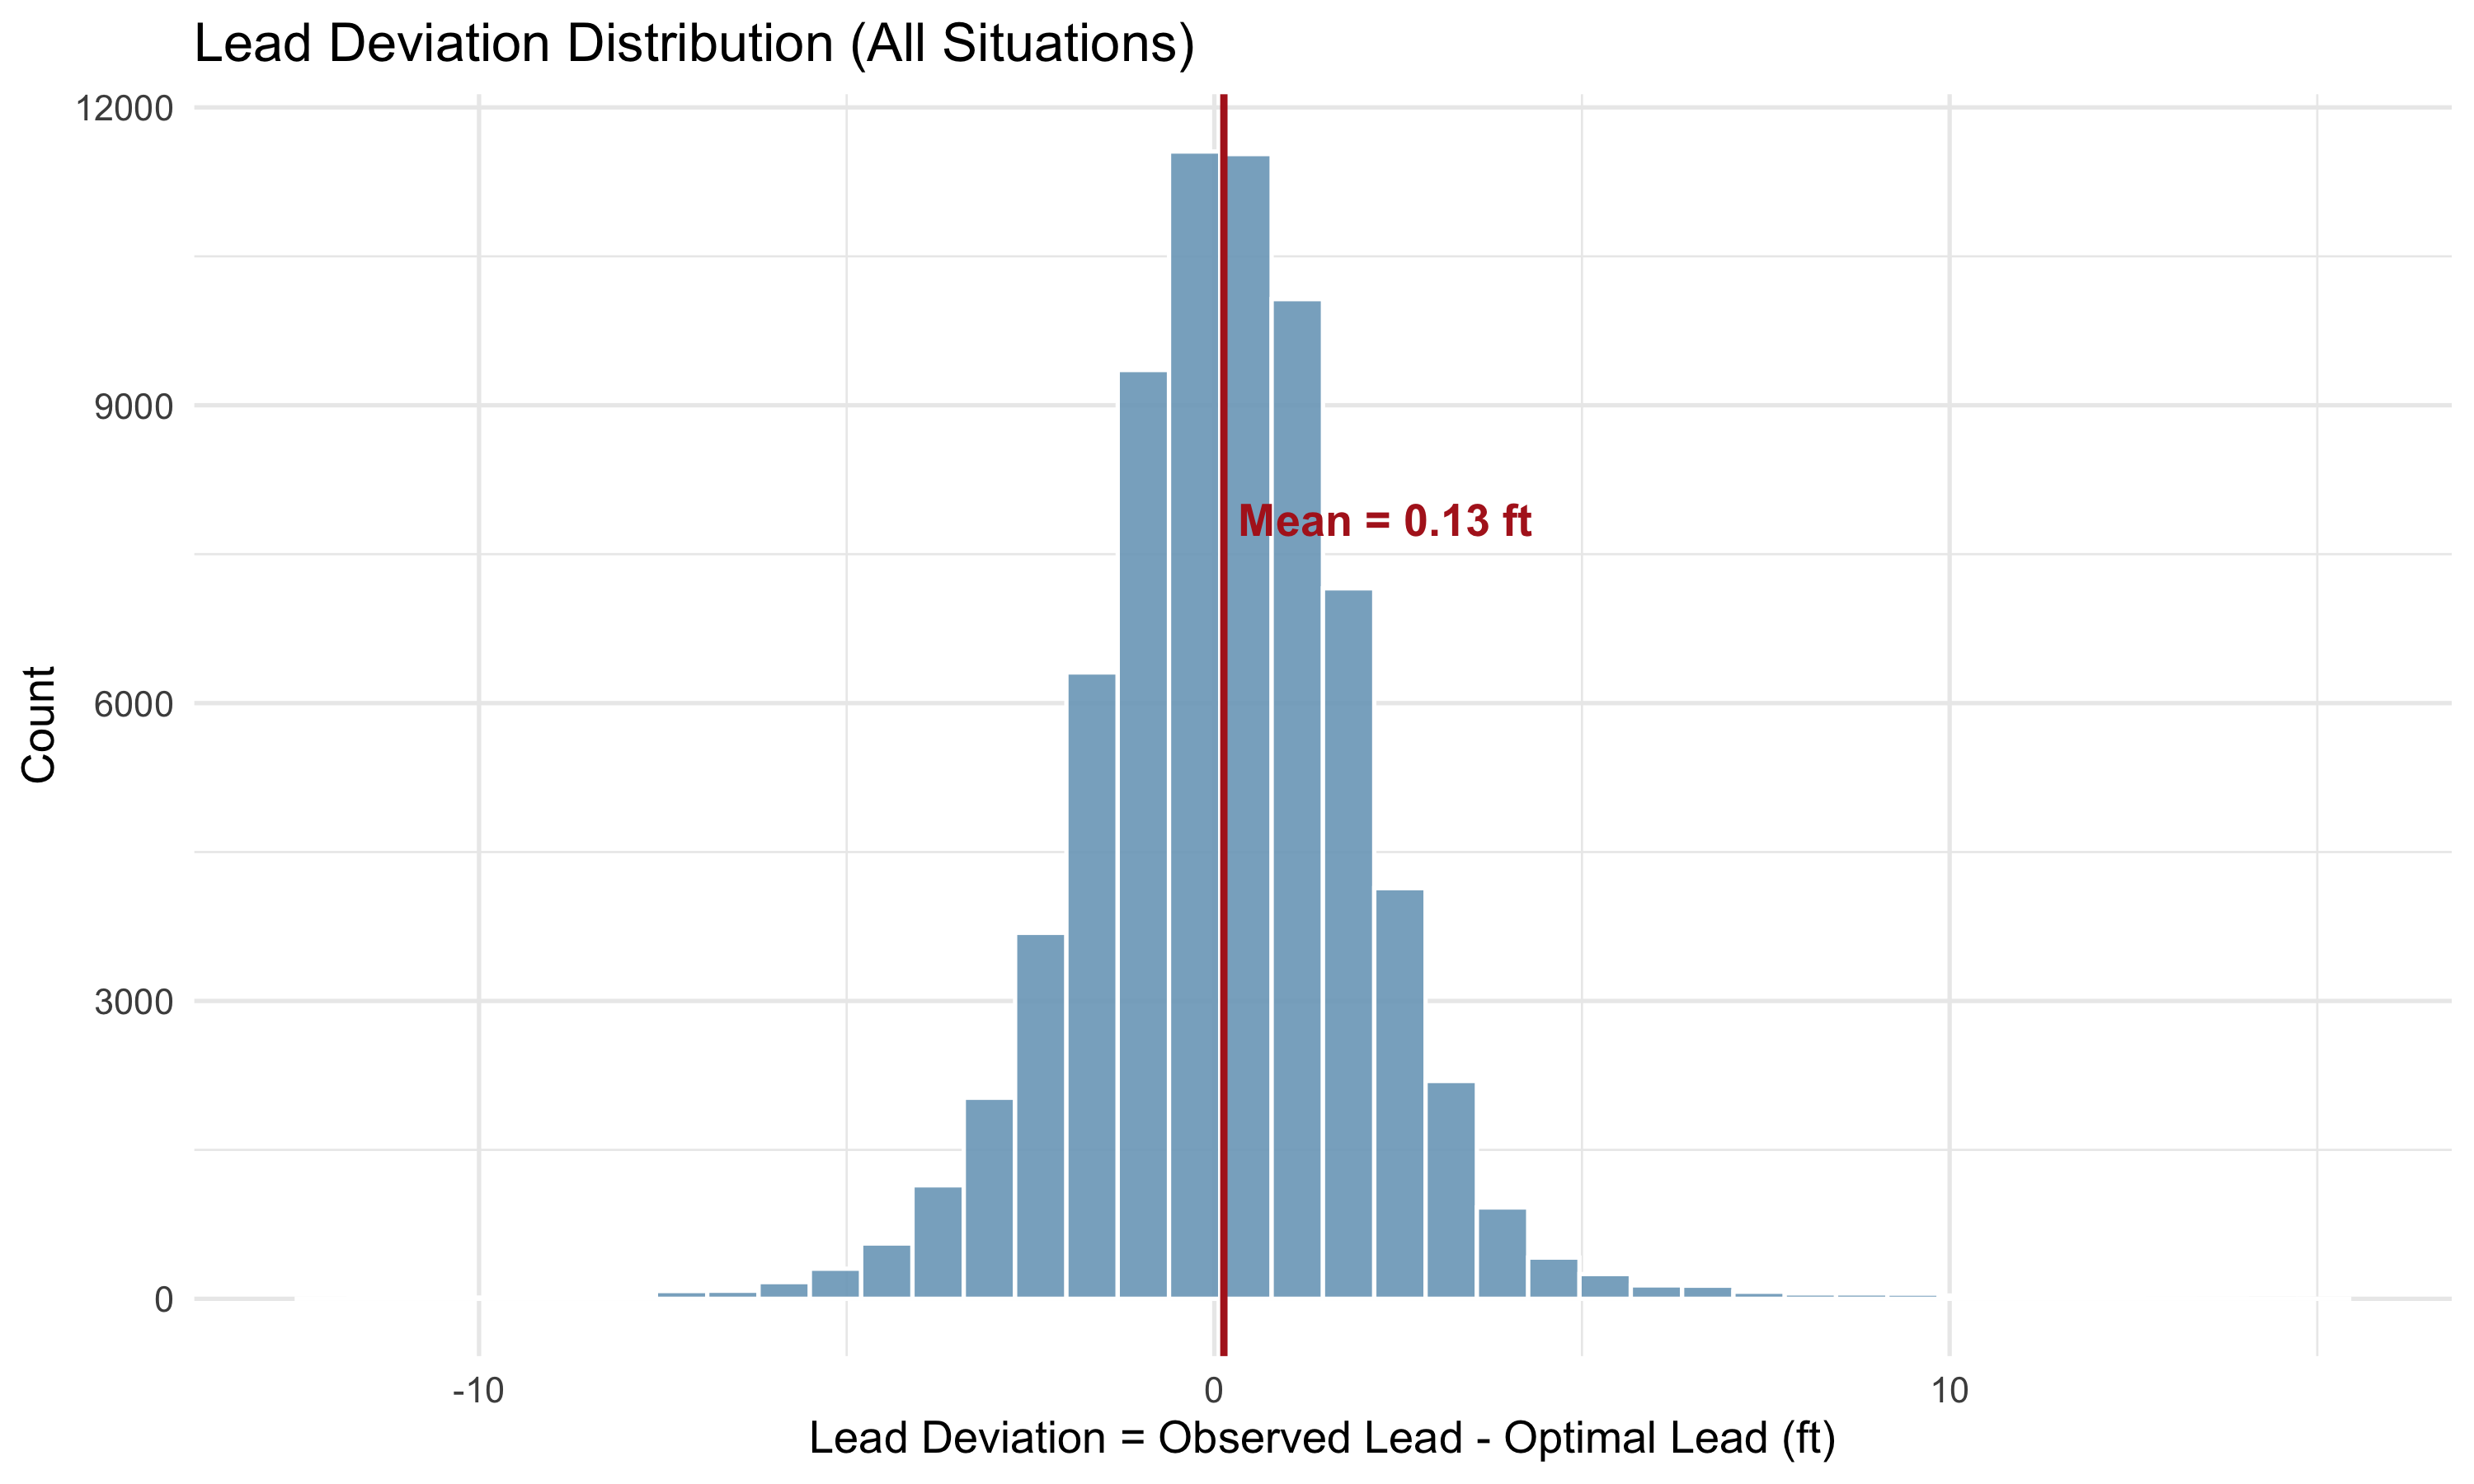
\includegraphics[width=0.8\textwidth]{figures/Lead-Error-All-MMNew.png}
    \caption{Distribution of lead deviations across all situations. Positive values indicate observed leads larger than the model-implied optimum; the red vertical line and label mark the sample mean (+0.13 ft).}
    \label{fig:deviation_all}
\end{figure}

\begin{figure}[!htbp]
    \centering
    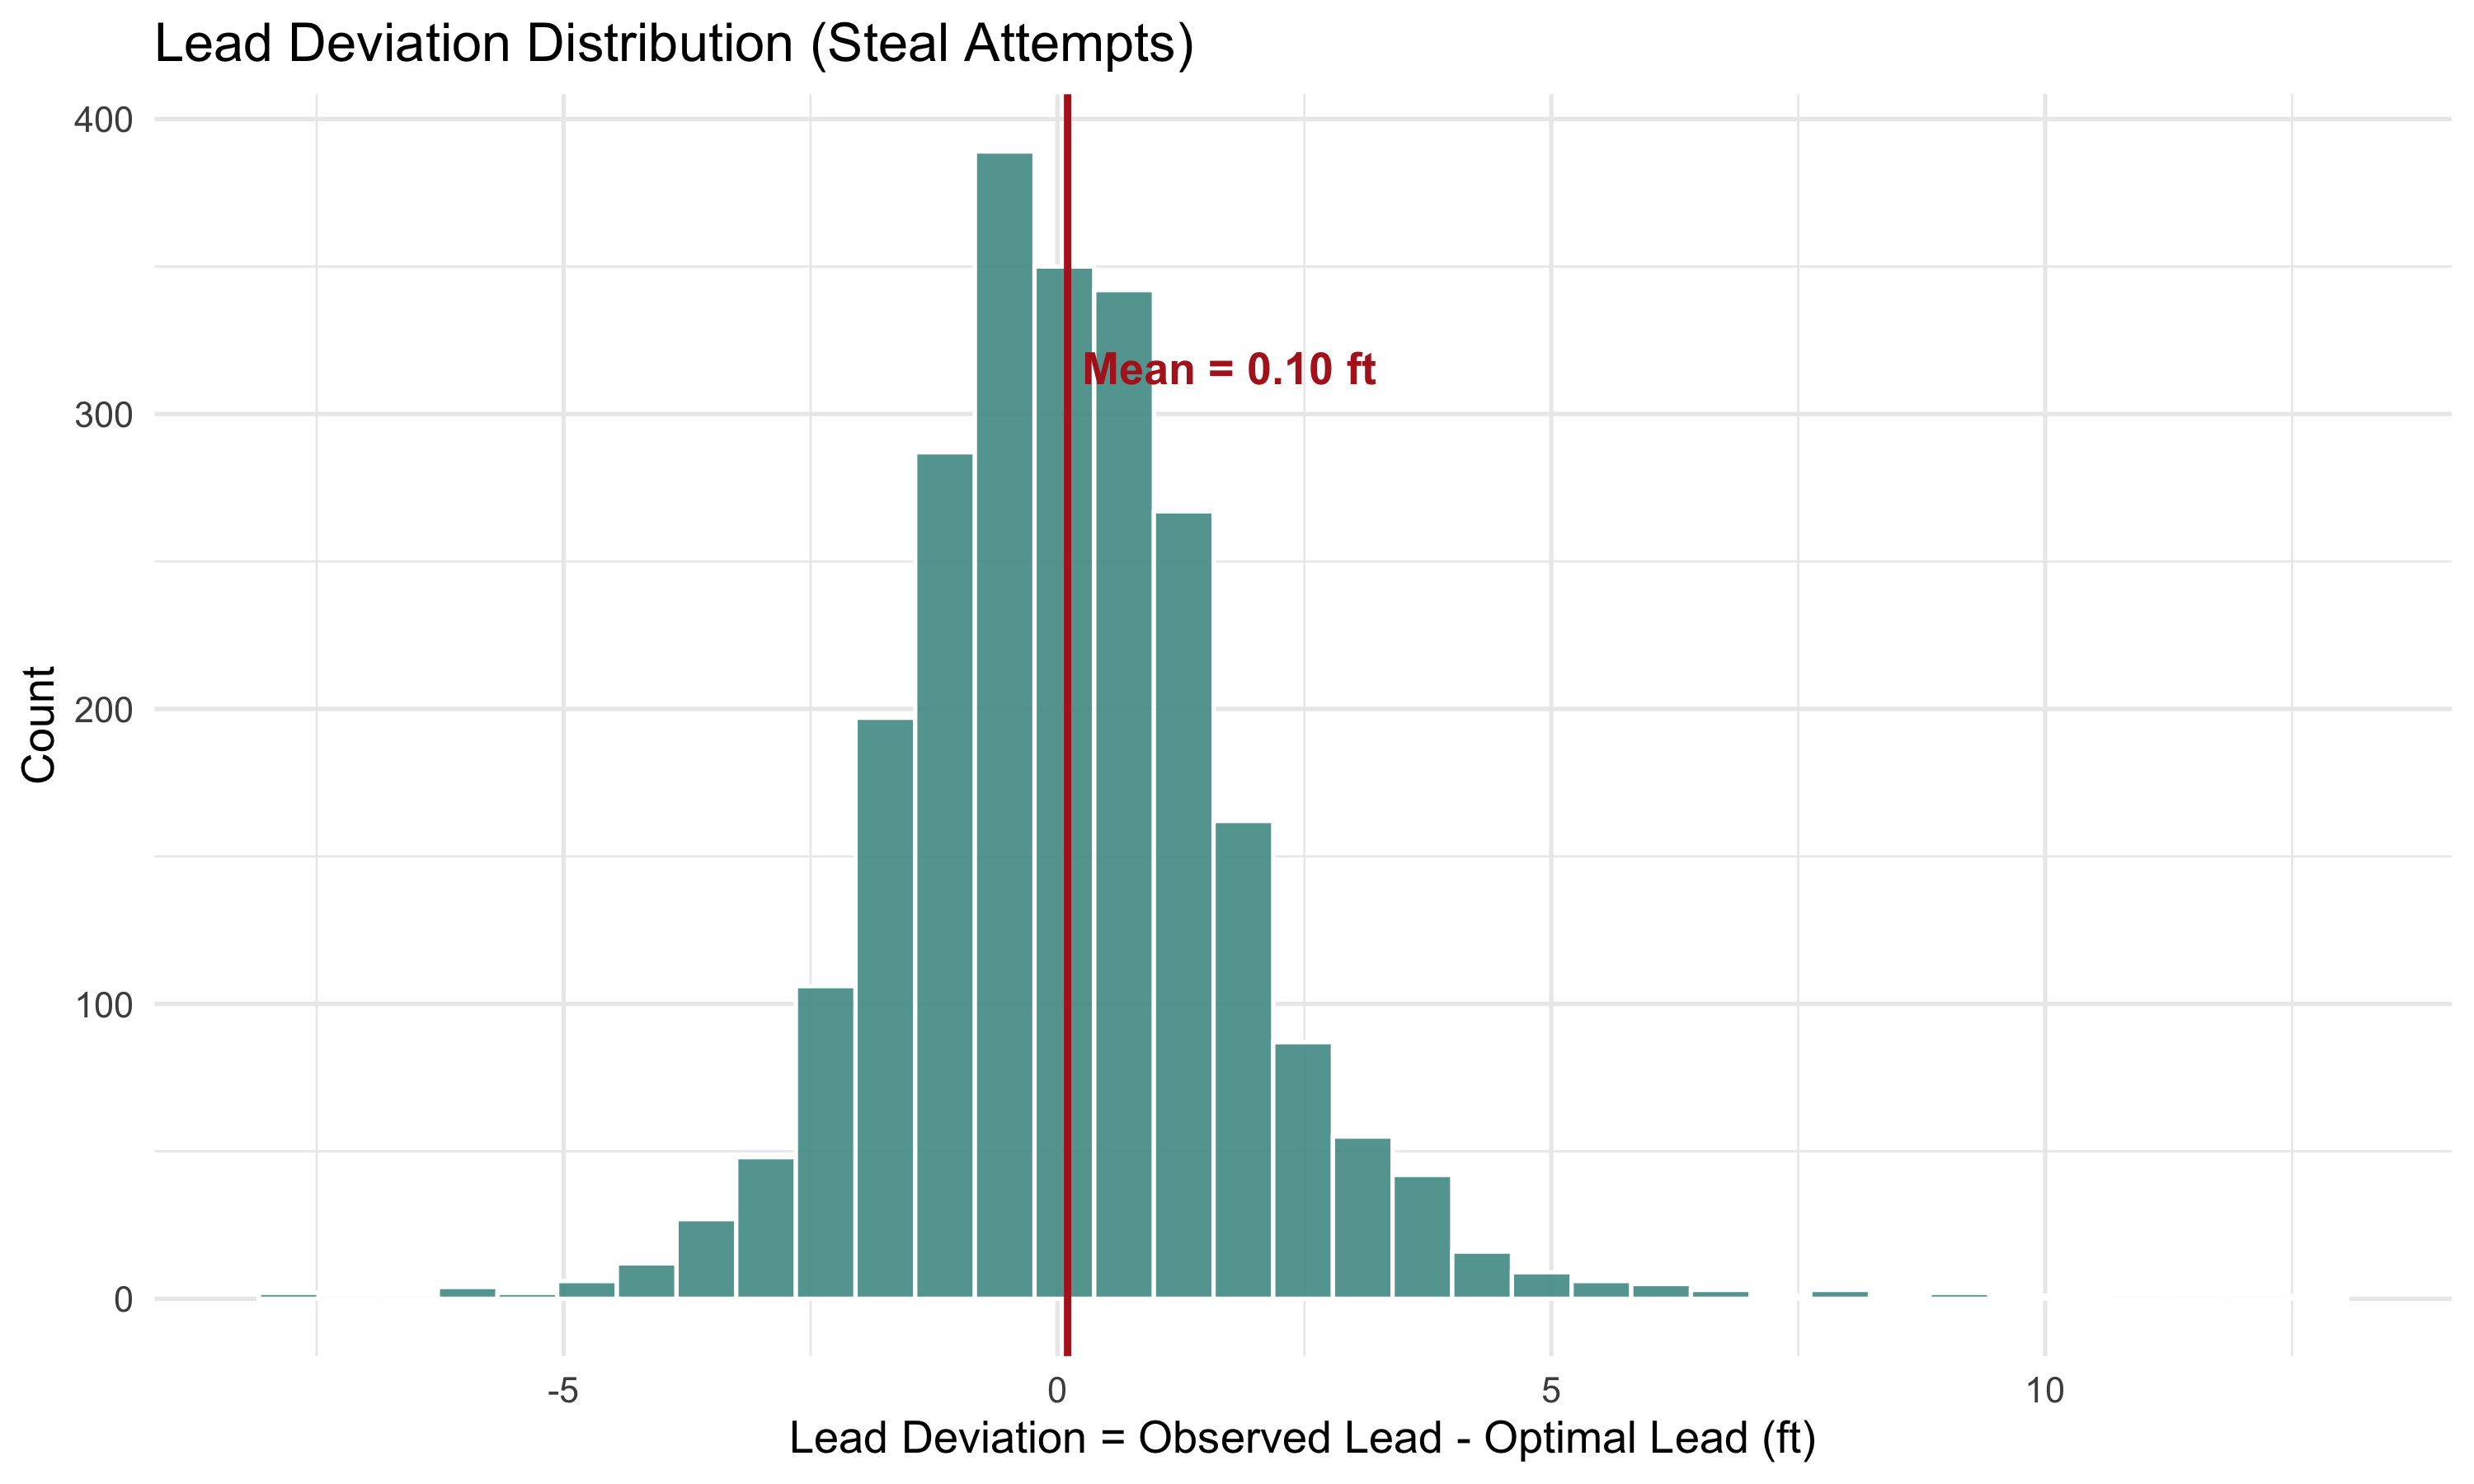
\includegraphics[width=0.8\textwidth]{figures/Lead-Error-SB-MMNew.png}
    \caption{Distribution of lead deviations when a stolen base is attempted. The mean remains positive but is lower than the all-situations mean; the red vertical line and label mark the sample mean (+0.10 ft).}
    \label{fig:deviation_sba}
\end{figure}

\subsection{Case Study: Cubs vs. Pirates, August 28, 2024}

In an August 28, 2024 game between the Chicago Cubs and Pittsburgh Pirates, Pete Crow-Armstrong (PCA) took an 11.46-foot lead against pitcher Paul Skenes and catcher Yasmani Grandal (Figure~\ref{fig:example_case}). Given PCA's sprint speed of 30 ft/s, Skenes's estimated Threat of 4.04, Grandal's pop time of 2.09 seconds, and the game context, the model produces an optimal lead estimate of $L_i^*=11.33$ ft. PCA's observed lead exceeds this estimate by 0.13 ft, indicating a slightly more aggressive lead than the model-implied optimum.

Figure~\ref{fig:implied_probs} displays the model-implied probabilities of SB, CS, and PK as functions of primary lead $L$, along with the expected run value $\mathrm{xRuns}(L\mid X_i)$. Figure~\ref{fig:optimal_lead} shows that a lead distance of 11.33 ft maximizes the estimated expected run value (+0.0122). This turning point reflects the lead-taking trade-off: larger leads increase the probability of reaching second safely, but eventually the increased pickoff risk dominates.

\begin{figure}[H]
    \centering
    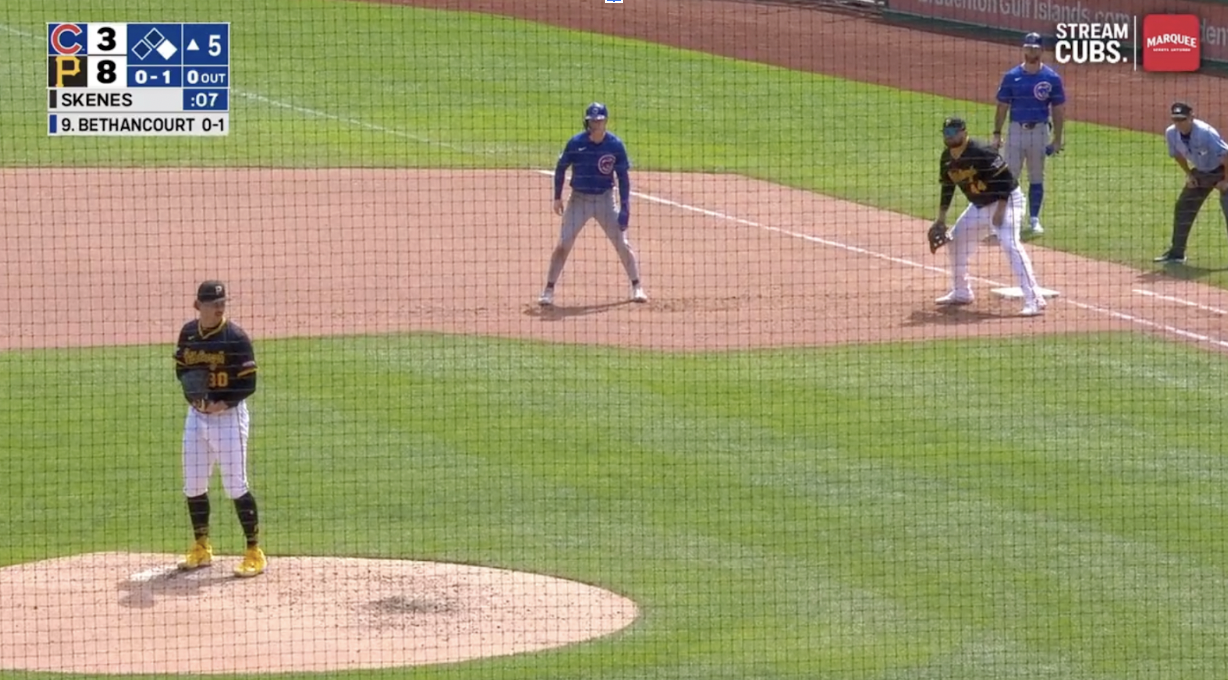
\includegraphics[width=0.9\textwidth]{figures/pca.png}
    \caption{Pete Crow-Armstrong on first base, Paul Skenes pitching, and Yasmani Grandal catching offscreen. \citep{CubsvPirates2024}}
    \label{fig:example_case}
\end{figure}

\begin{figure}[H]
    \centering
    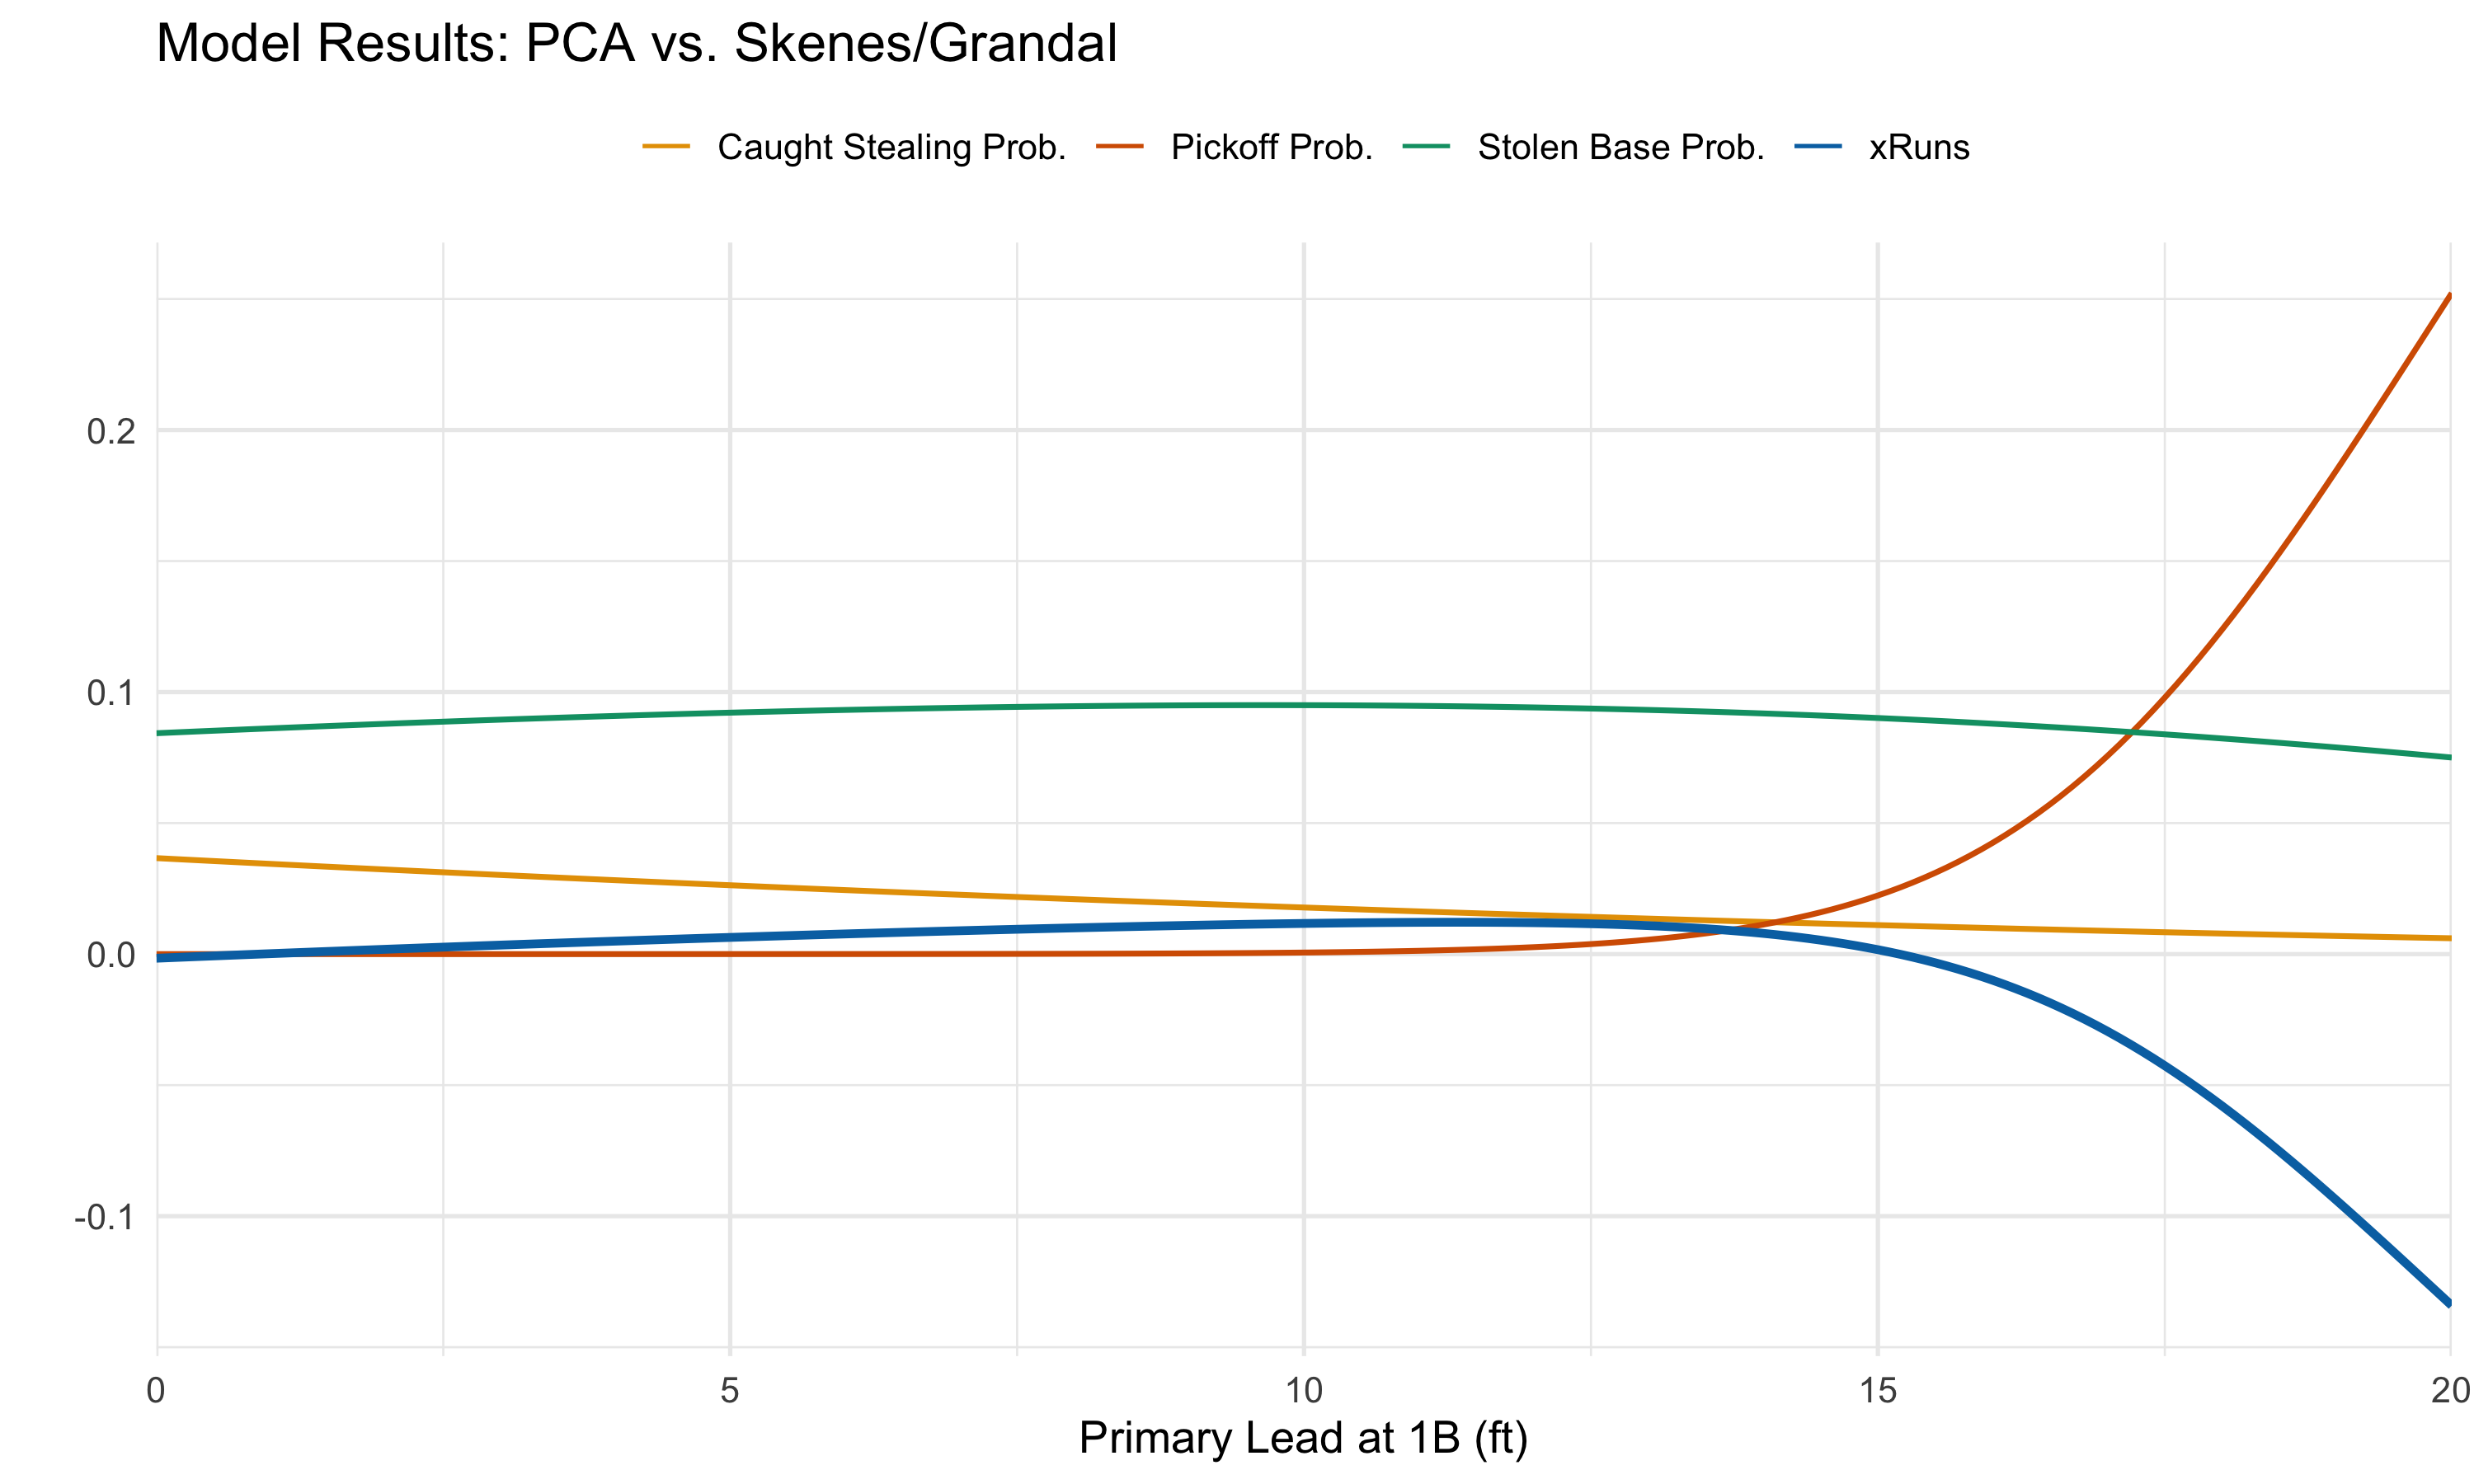
\includegraphics[width=0.9\textwidth]{figures/pca-probs-MMNew.png}
    \caption{Model-implied outcome probabilities and estimated expected run value as functions of Pete Crow-Armstrong's primary lead distance. Probabilities and expected run value are shown on the same axis for visual comparison.}
    \label{fig:implied_probs}
\end{figure}

\begin{figure}[H]
    \centering
    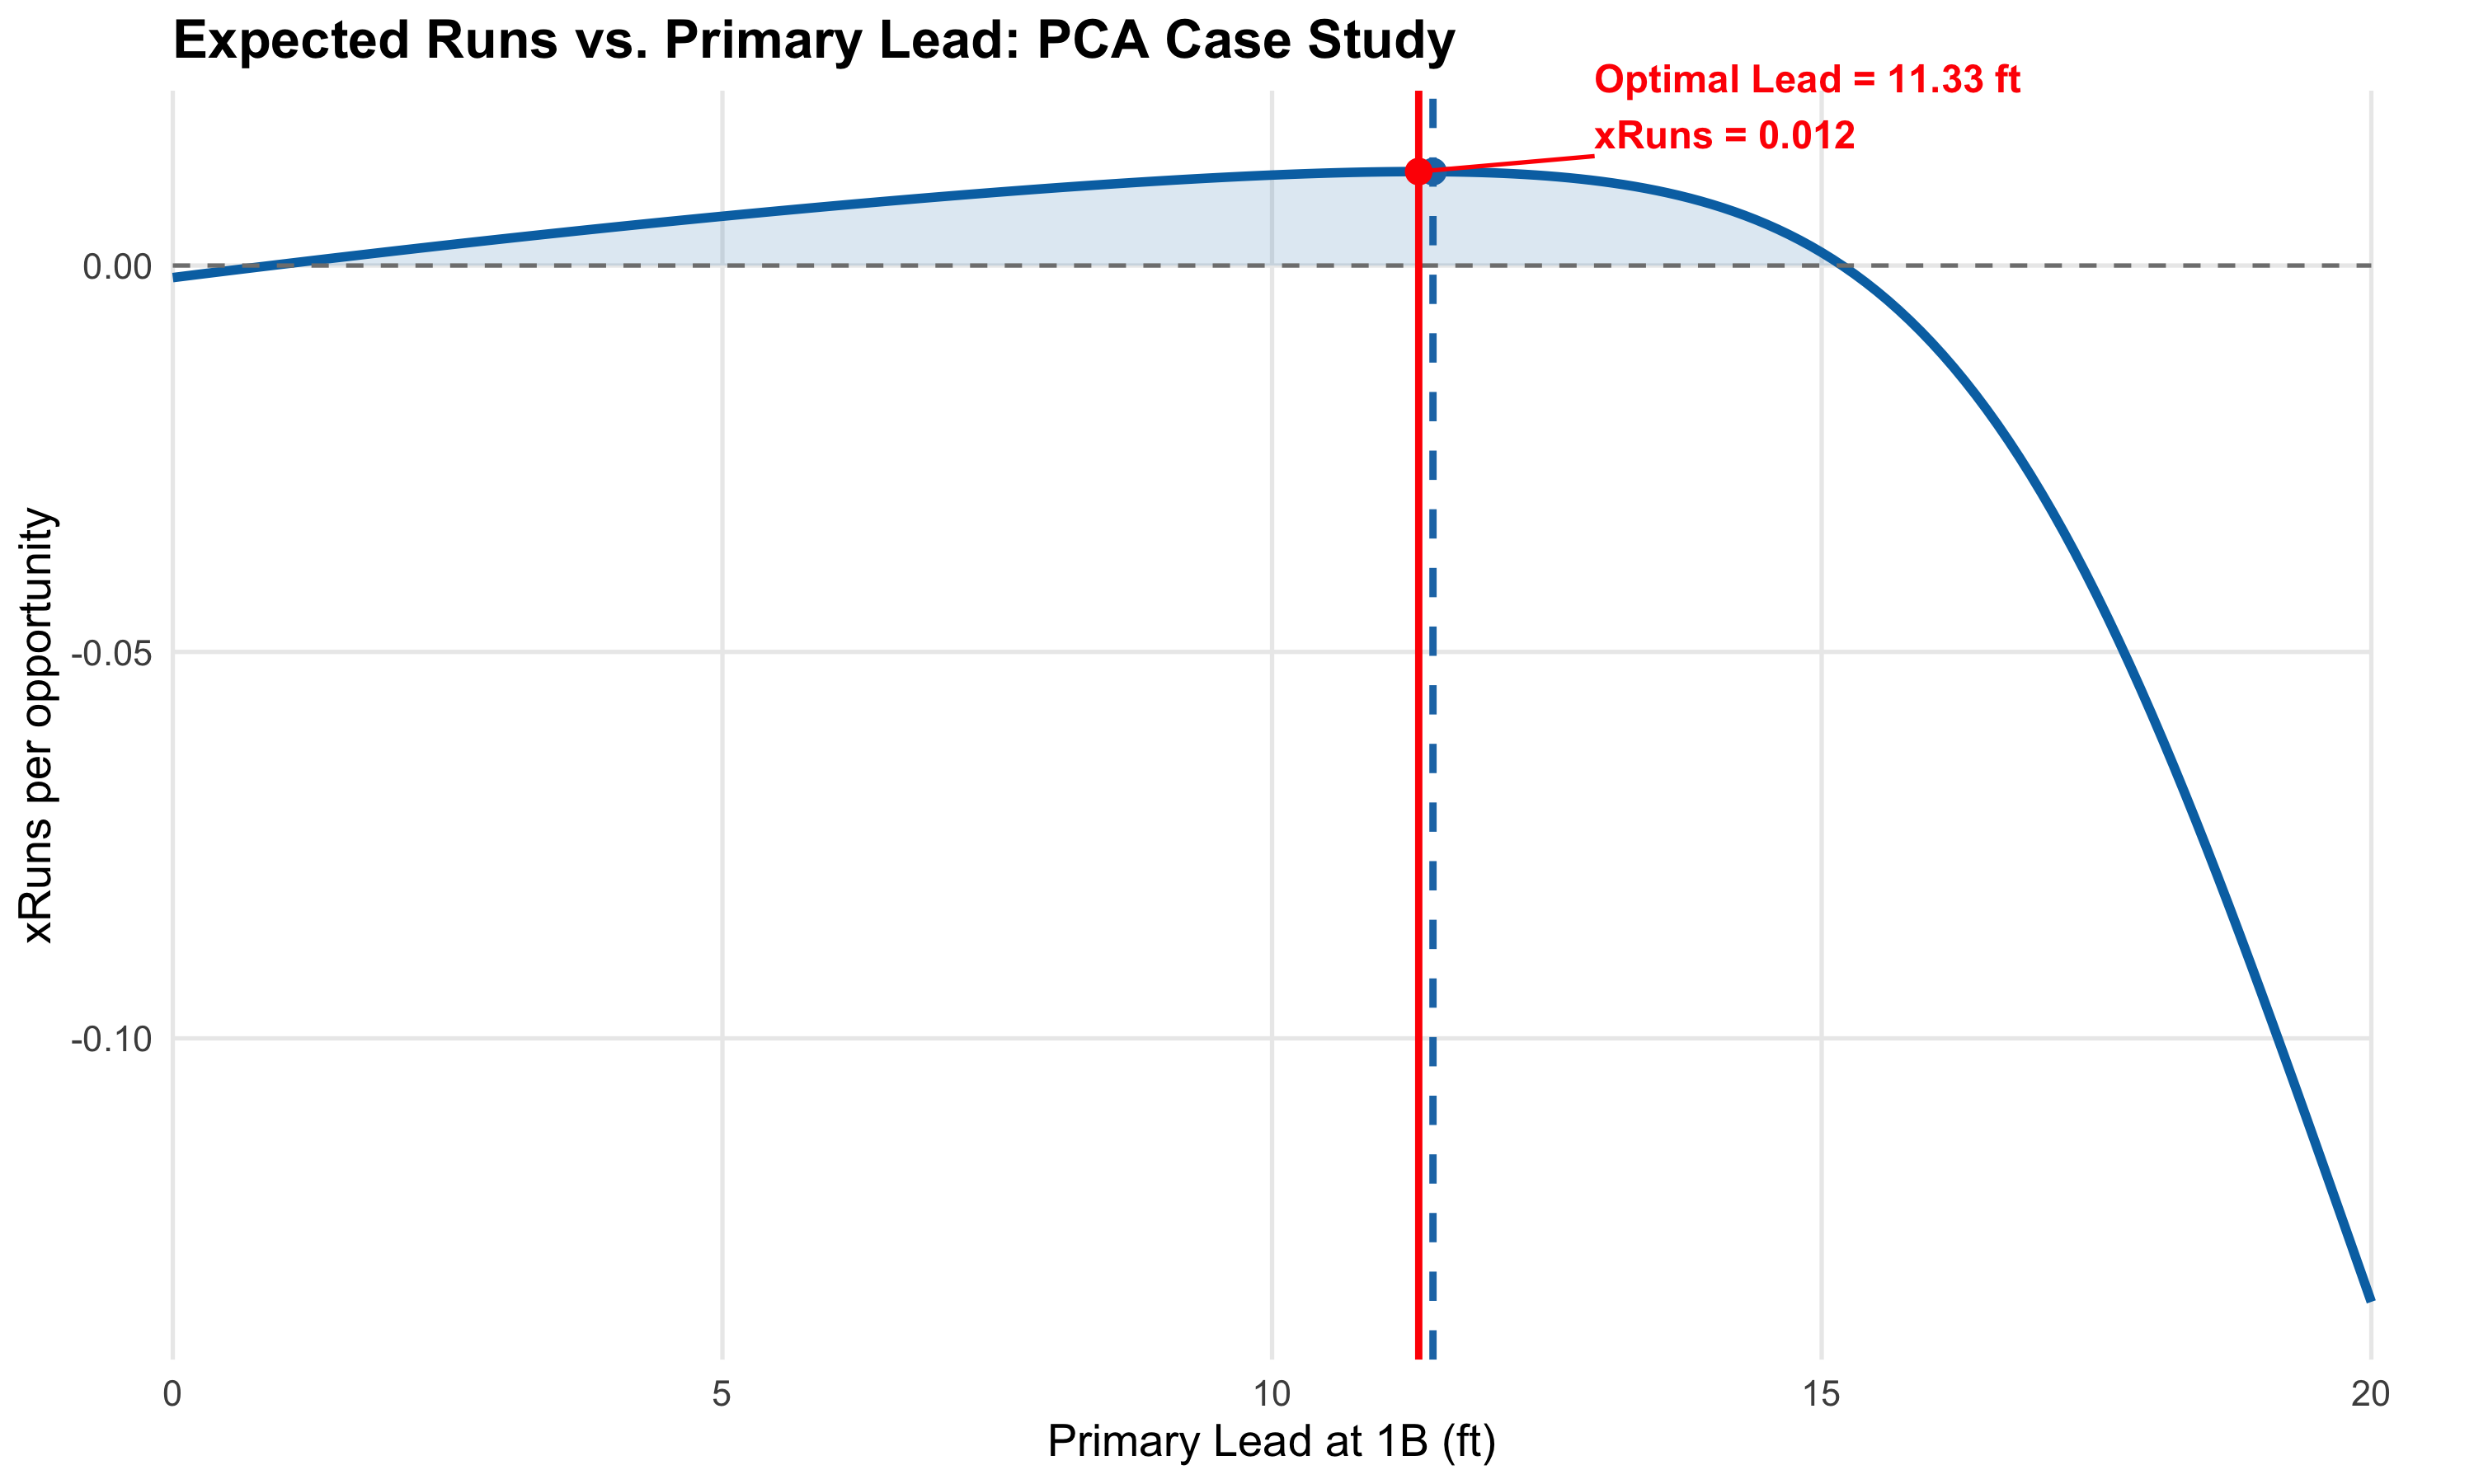
\includegraphics[width=0.9\textwidth]{figures/pca-xruns-MMNew.png}
    \caption{Estimated expected run value as a function of Pete Crow-Armstrong's primary lead distance. The red marker denotes the model-implied optimal lead, and the blue dashed marker denotes PCA's observed lead in the play.}
    \label{fig:optimal_lead}
\end{figure}

\section{Discussion}

\subsection{Conclusions}

This study proposes a framework for estimating primary lead distances off first base that maximize expected runs in the base state with a runner on first and second and third base empty. We model the baserunning sequence with a nested logistic and mixed-effects logistic stack, using runner sprint speed, catcher pop time, pitcher hold ability (\emph{Threat}), disengagement stage, outs, and runner/catcher random effects in the relevant stages. By mapping stage probabilities to RE24 run values, we obtain a context-specific model-implied optimal lead $L_i^*$ and a diagnostic measure of deviation, $L_i^{\mathrm{obs}}-L_i^*$.

The fitted models capture the core trade-off in lead-taking. Increasing lead length is associated with higher steal-success probability but also with greater pickoff exposure, producing an expected run value profile with an interior maximum in the PCA case study and in the contexts considered here. Empirically, observed leads are modestly larger than the model-implied optimum on average ($\approx$ +0.13 ft), while steal attempts show a smaller positive deviation ($\approx$ +0.10 ft). The positive sign indicates that runners in this sample are, on average, slightly more aggressive than the model-implied optimum, though the magnitude is small.

These findings offer an interpretable, data-driven basis for calibrating lead size. Rather than evaluating steals and pickoffs separately, the method places the full steal--pickoff trade-off on a common run-expectancy scale and produces context-specific recommendations within the range supported by the data.

\subsection{Limitations and Future Directions}

The analysis has several limitations. First, we do not observe steal intent on a given pitch. Lead distance may therefore proxy for unobserved green-light decisions, especially on pitches where the runner was planning to go. We partially address this by excluding lead distance from the steal-attempt model, but direct intent labels would allow a cleaner separation between strategic intent and realized positioning.

Second, the fitted probabilities should be interpreted as model-implied quantities for the analyzed pitch sample rather than as fully calibrated league-wide event probabilities. This point mainly affects the level of the expected run value function, not the qualitative logic of the trade-off, but it is important when interpreting the numerical optimum as a recommendation.

Third, the disengagement variable is constructed from observed pickoff attempts only. Because step-offs are not observed, this variable may understate the true number of disengagements in a plate appearance.

Fourth, we restrict attention to the base state with a runner on first and second and third empty. Other base states would change both the RE24 payoffs and defensive behavior. Extending the model to all base-out states is a natural next step.

Finally, the current model treats pitches as conditionally independent. In practice, pitchers, runners, and catchers adapt within plate appearances and across games. A dynamic model with plate-appearance history, pitch type, batter handedness, pitch location, score, inning, and leverage could better capture this strategic interaction.

\subsection{Reproducibility}

All analysis code and figure scripts are available
\href{https://github.com/wharton-moneyball/stolen-base-leads}{here}. Proprietary MLB data are not publicly available.

\section{Acknowledgments}

We would like to thank Moneyball Academy, led by Professor Abraham Wyner and the Wharton Sports Analytics and Business Initiative (WSABI), for supporting this research. We are also grateful to Major League Baseball for providing the data. We thank Jonathan Pipping, Noah Sonnenklar, and Adam Kuechler for their mentorship and guidance, and our teammates, Will Diflorio and Jackson Hubbard, for their contributions over the summer.

\bibliographystyle{apalike}
\bibliography{references}

\clearpage
\appendix

\begin{center}
\Large\bfseries Appendix
\end{center}

\section{Additional Lead Deviation Visualizations} \label{app:a}

Figure~\ref{fig:deviation_by_team} reports the mean absolute lead deviation by team across all runner-on-first events. Lower values indicate closer adherence to the model-implied optimal lead. In this sample, the New York Yankees exhibit the largest mean absolute deviation by a substantial margin (about 0.61 ft above the next highest team), whereas the Cleveland Guardians and Seattle Mariners exhibit the lowest deviations.

All runner lists below include only players with at least 15 observations. These plots should be read as exploratory summaries rather than definitive rankings, since the estimates do not include uncertainty intervals. Figure~\ref{fig:runners_closest} displays the runners with the smallest absolute mean lead deviation. Figures~\ref{fig:runners_aggressive} and~\ref{fig:runners_conservative} show the tails of the signed distribution: the former lists runners with the most positive average deviations, and the latter lists runners with the most negative average deviations. Jahmai Jones, Ryan O'Hearn, and Nelson Velazquez are closest to the model-implied optimum on average. Daniel Vogelbach, Wilmer Flores, and Brandon Crawford take the most aggressive leads on average, while Brooks Baldwin, Anthony Volpe, and Juan Soto take the most conservative leads on average.

\begin{figure}[!htbp]
    \centering
    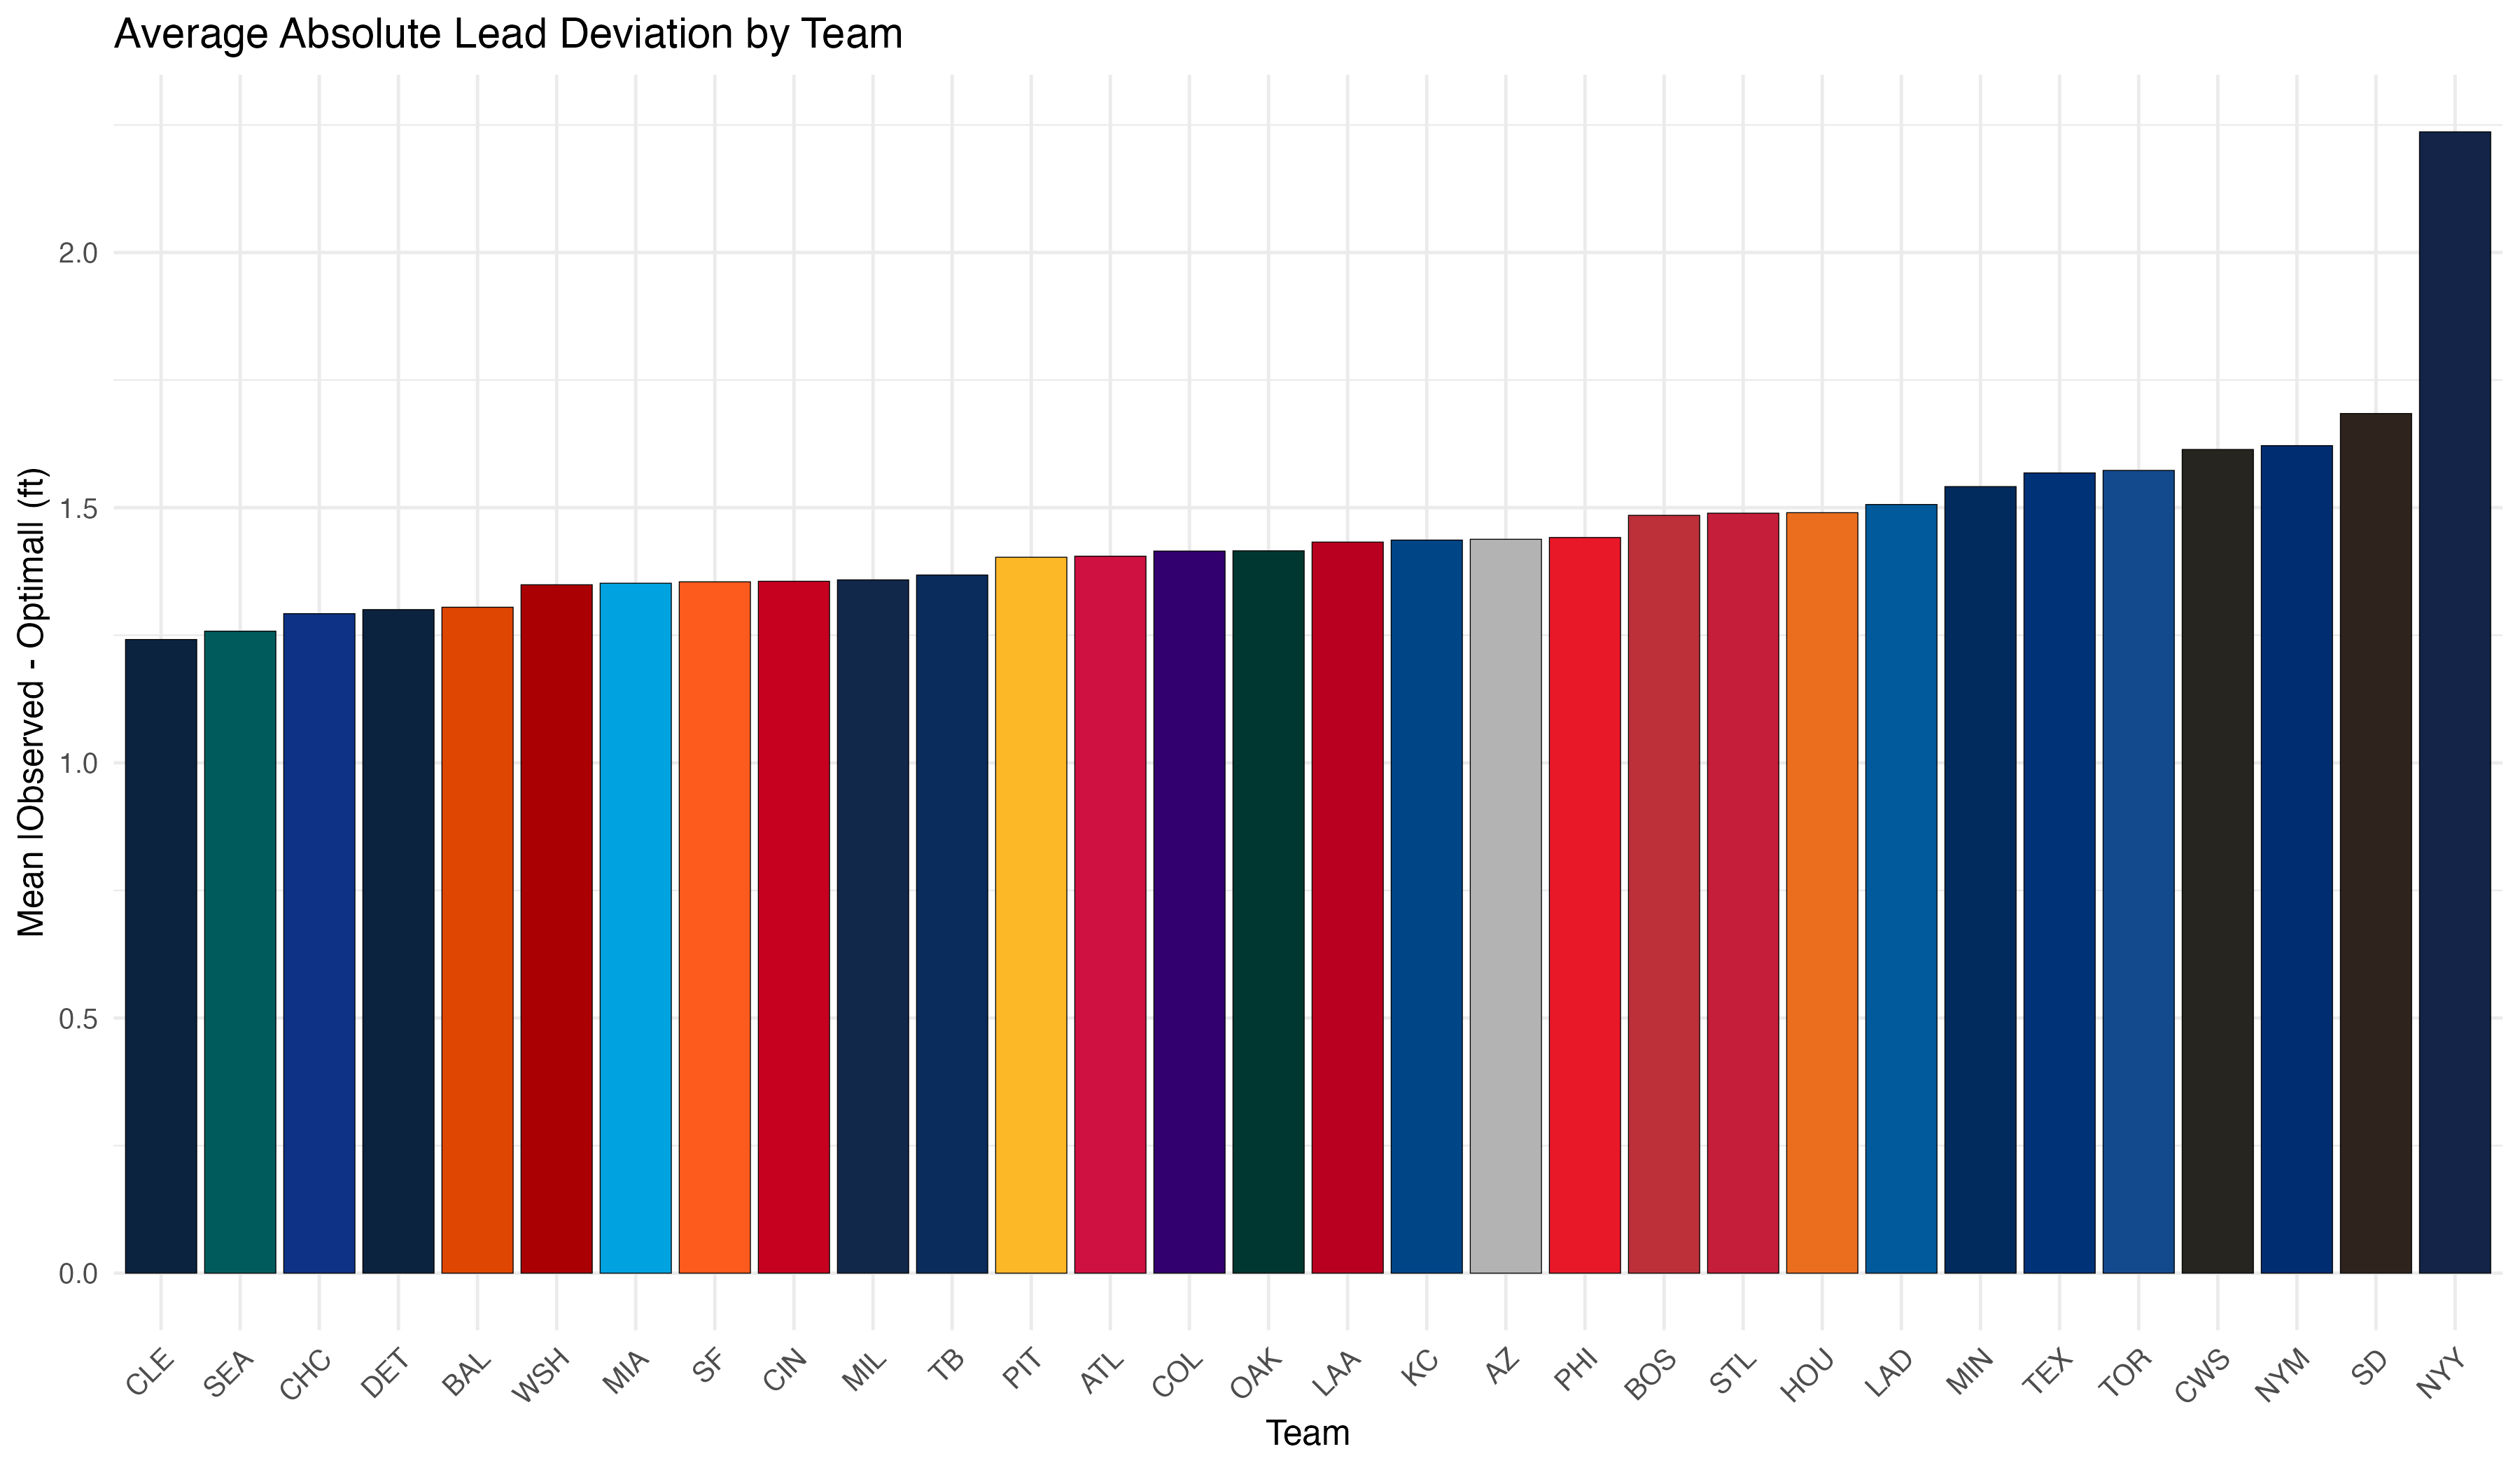
\includegraphics[width=0.9\textwidth]{figures/team-error-lead-MMNew.png}
    \caption{Average absolute lead deviation by team. Lower values indicate observed leads that are closer to the model-implied optimum on average.}
    \label{fig:deviation_by_team}
\end{figure}

\begin{figure}[!htbp]
    \centering
    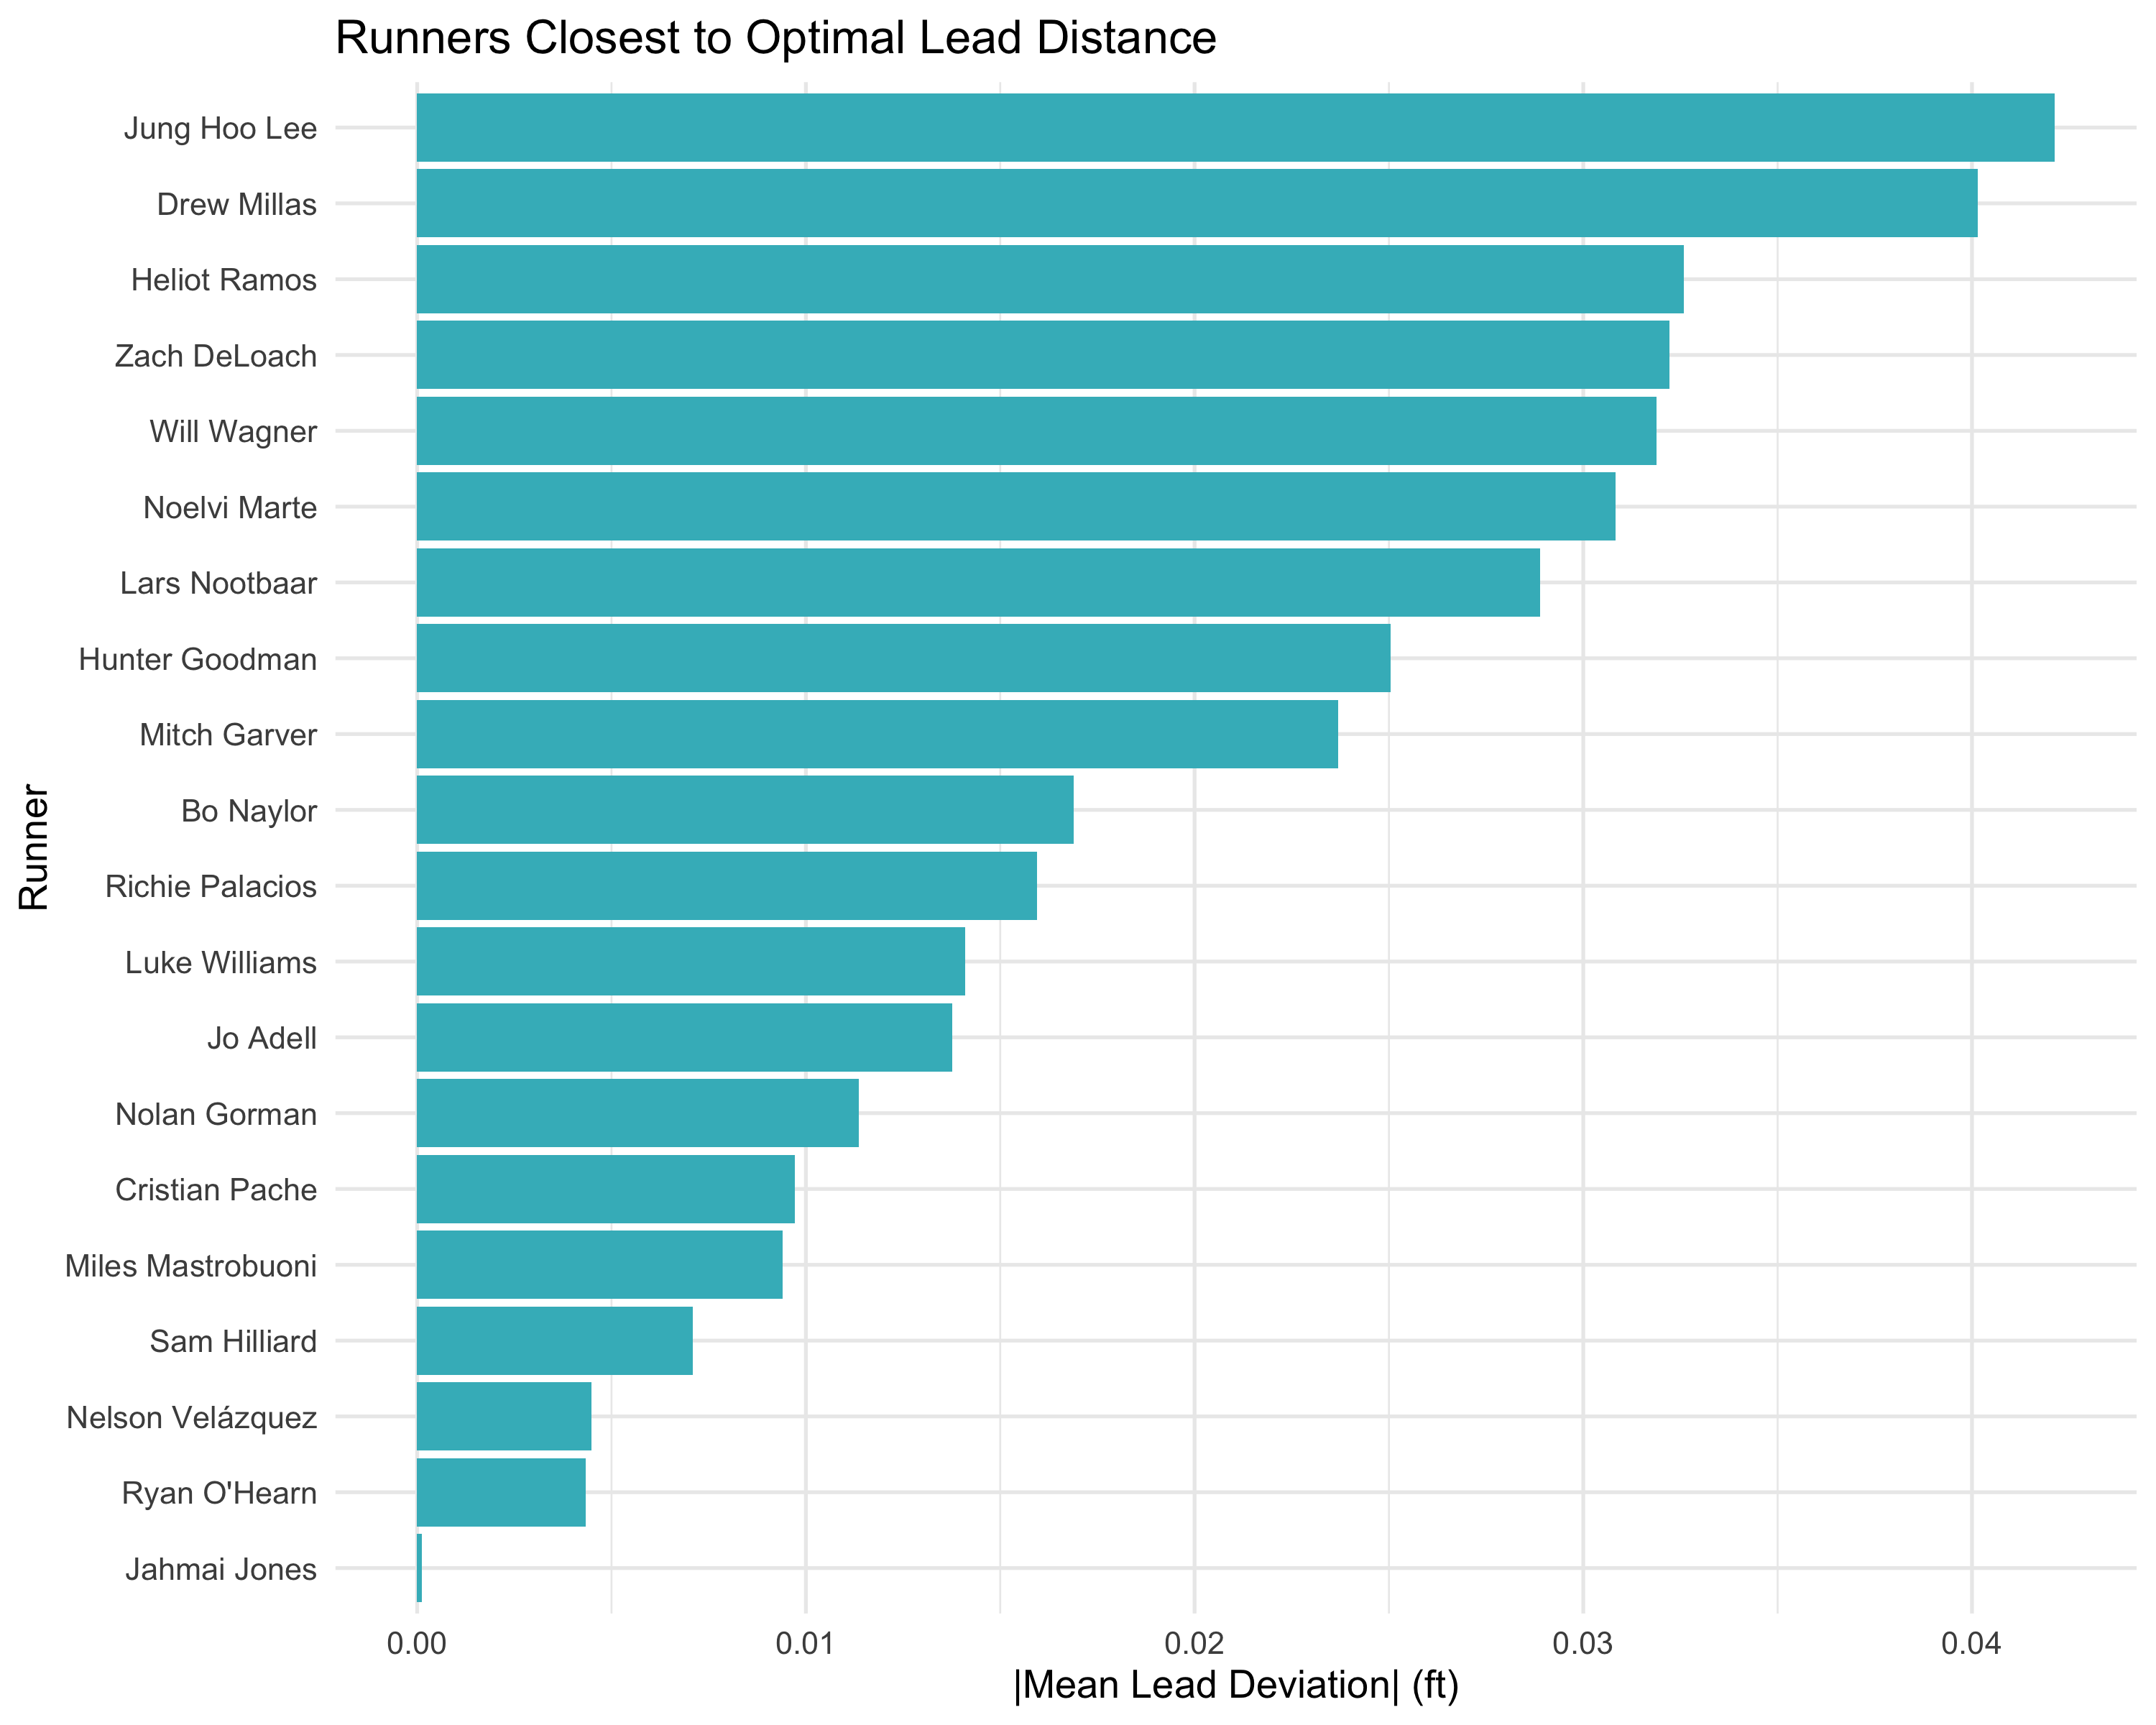
\includegraphics[width=0.8\textwidth]{figures/closest_to_optimal_leads.png}
    \caption{Baserunners with the smallest absolute average lead deviation among runners with at least 15 observations.}
    \label{fig:runners_closest}
\end{figure}

\begin{figure}[!htbp]
    \centering
    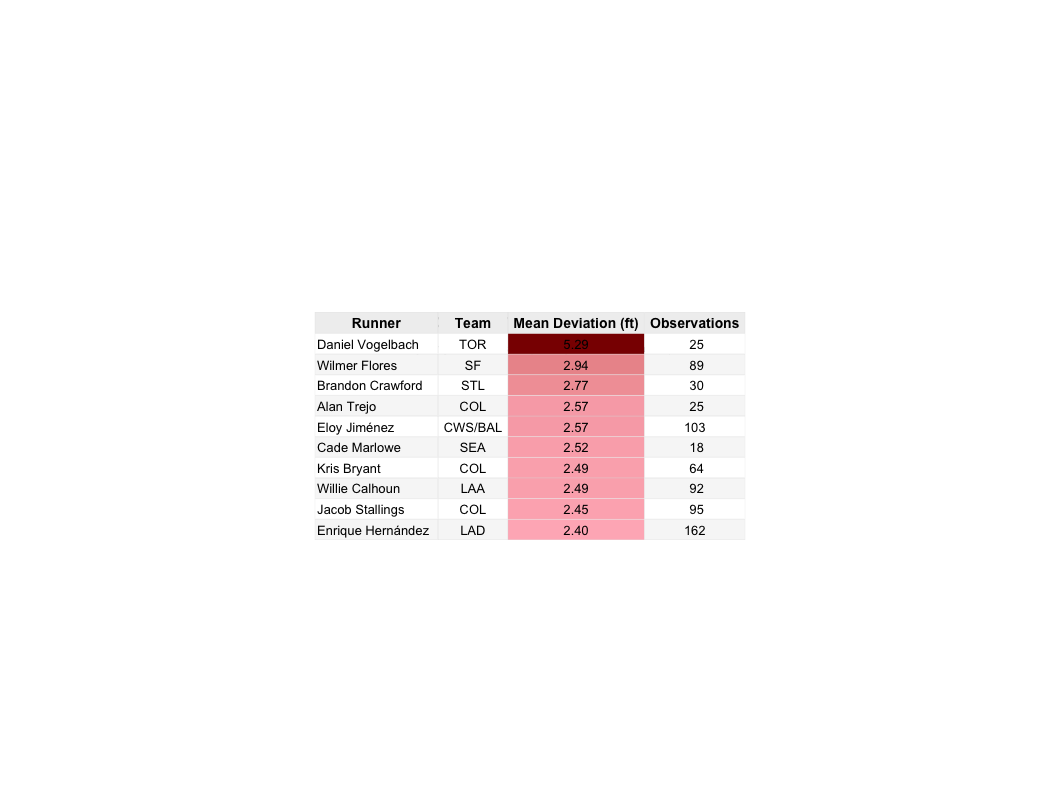
\includegraphics[width=0.75\textwidth]{figures/aggressive_leads.png}
    \caption{Baserunners with the most positive average lead deviations. Positive deviations indicate observed leads larger than the model-implied optimum.}
    \label{fig:runners_aggressive}
\end{figure}

\begin{figure}[!htbp]
    \centering
    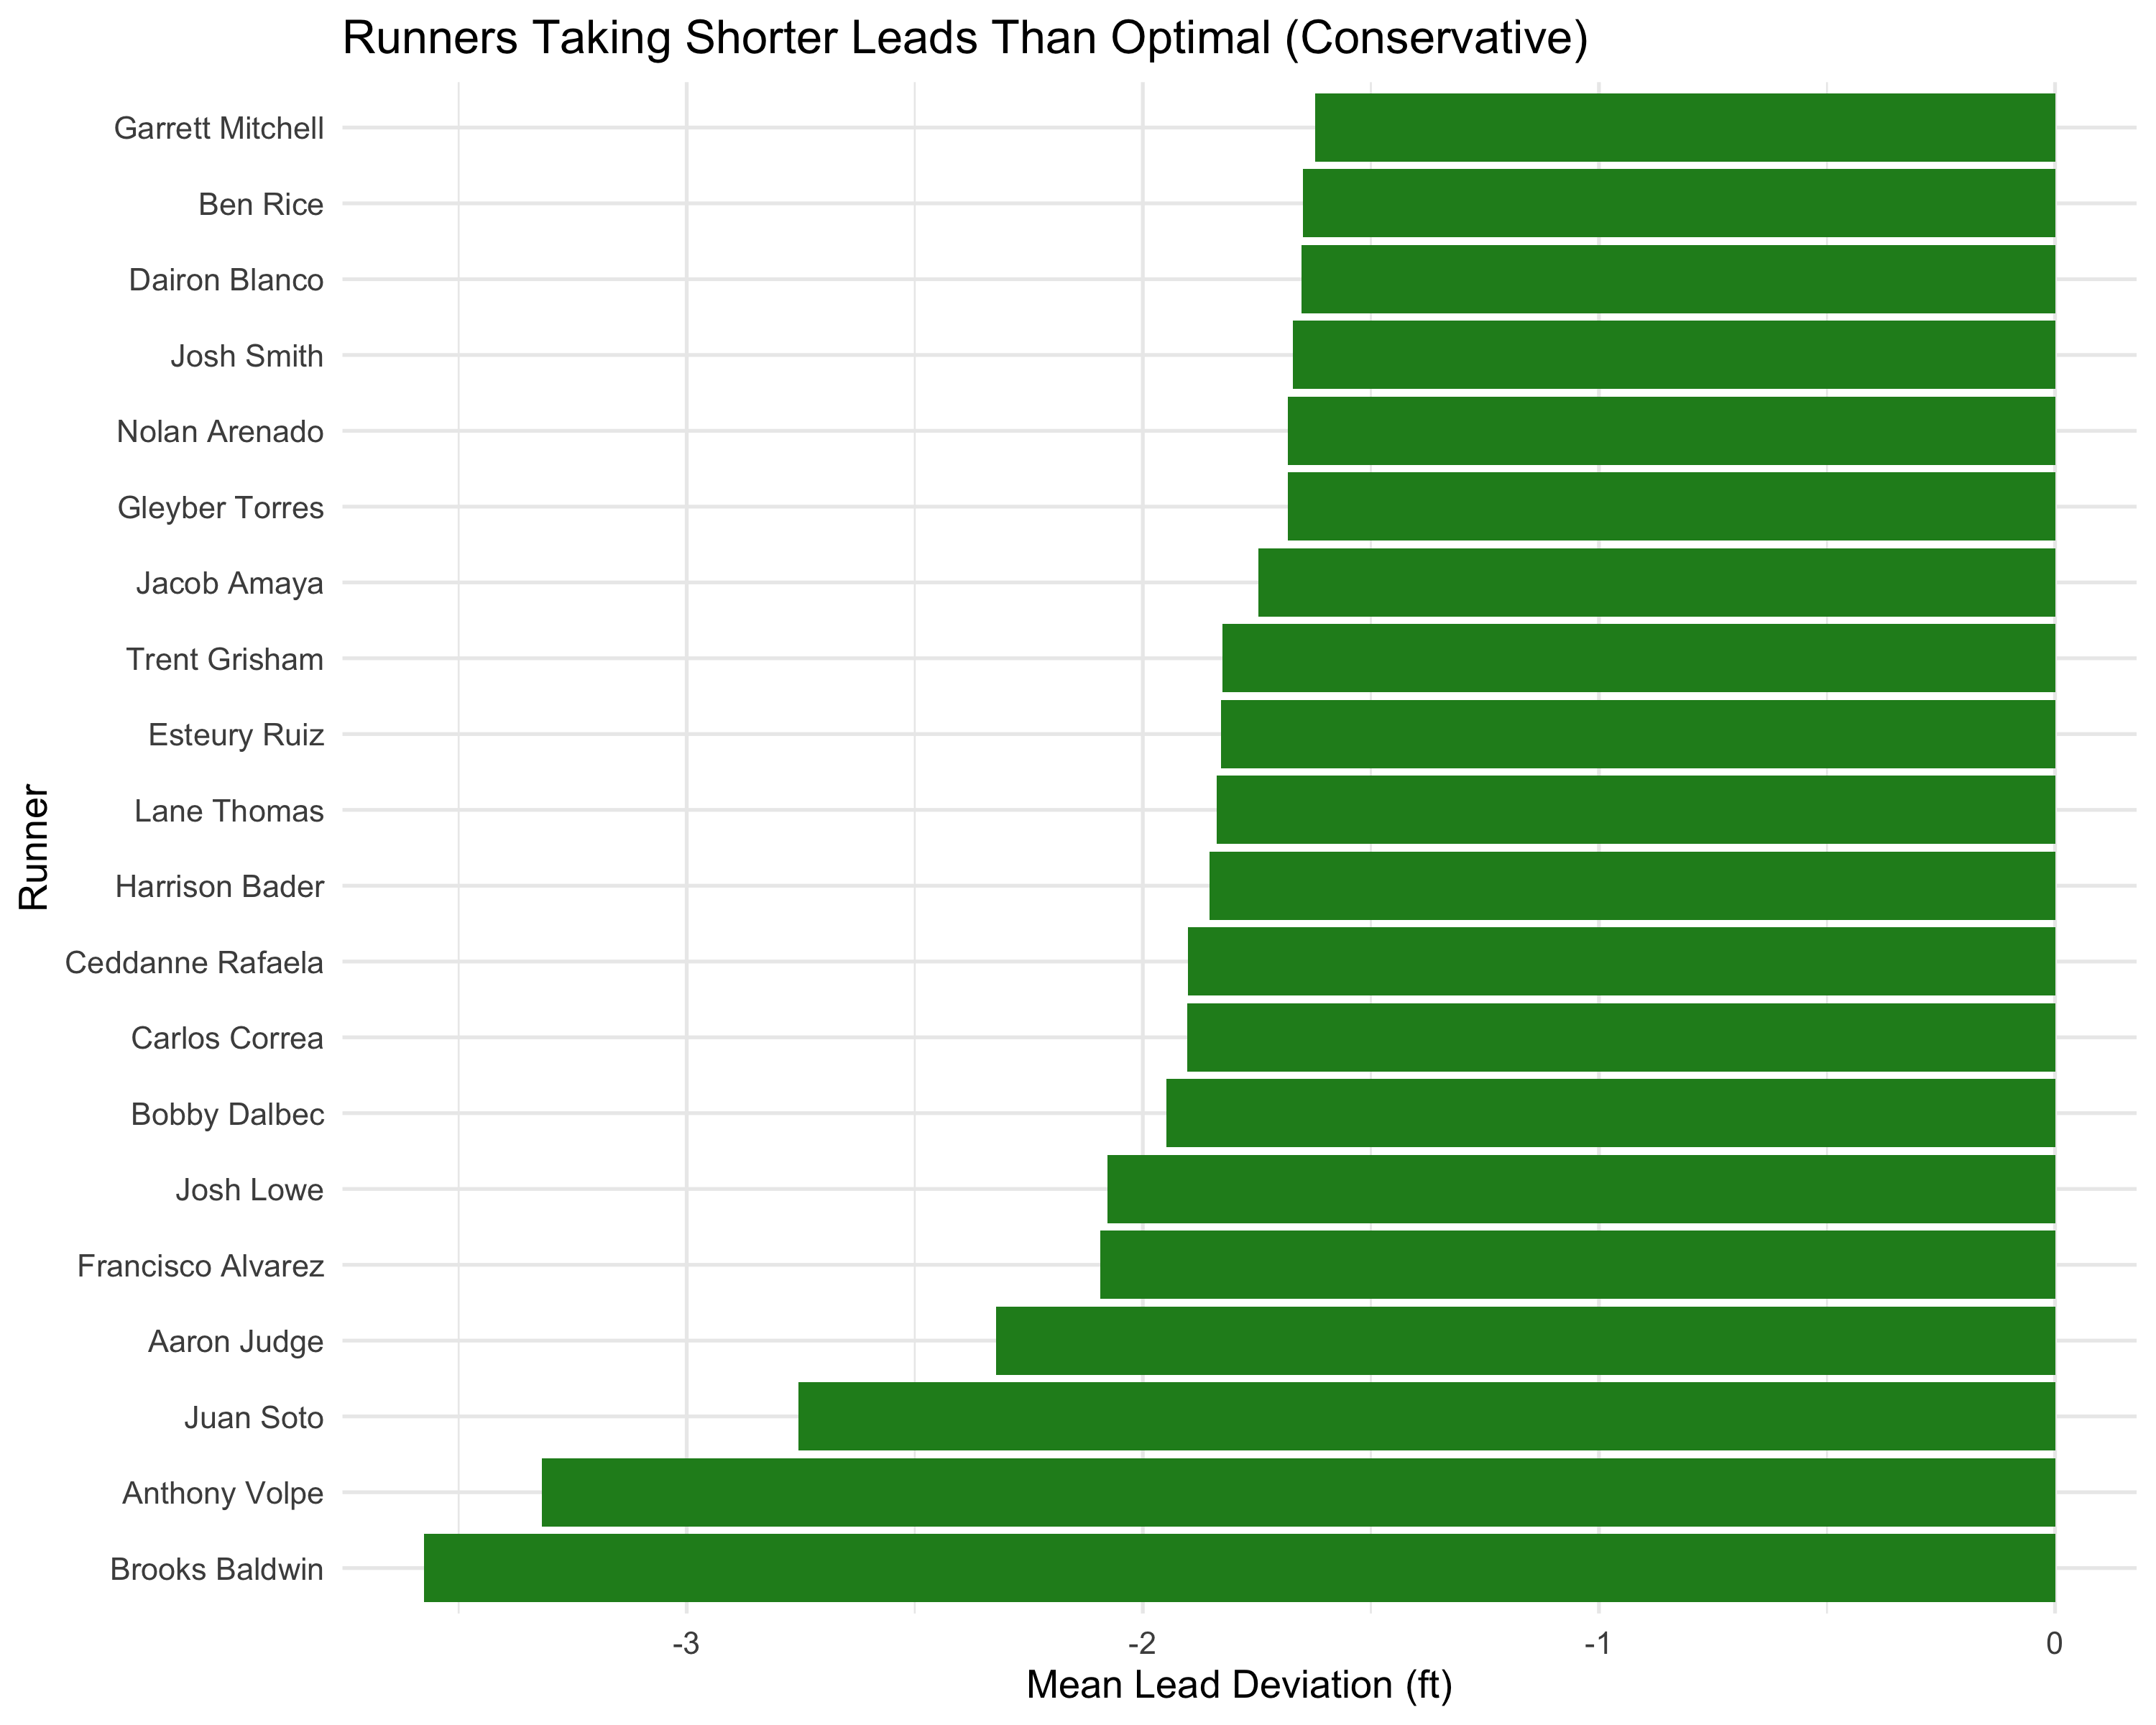
\includegraphics[width=0.75\textwidth]{figures/conservative_leads.png}
    \caption{Baserunners with the most negative average lead deviations. Negative deviations indicate observed leads smaller than the model-implied optimum.}
    \label{fig:runners_conservative}
\end{figure}

\end{document}
